\chapter{Image Processing Algorithms on Heterogeneous Platforms }
\label{sec:HCNN}

Feature extraction algorithms and Convolutional Neural Networks (CNN) are widely used in various problem domains, such as object detection, image classification, and segmentation. Feature Extraction  are typically designed to identify and extract relevant patterns or features from the input data. These algorithms are typically designed and implemented on DSPs or GPUs, which offer a specialised architecture properties which include thousands of general compute cores and coupled with a large amount of high-bandwidth memory. 

In the case of CNNs that contain millions of parameters, which in turn require significant memory resources to store their weights, implementing them on low-resource and energy constrained platforms is limited. Heterogeneous platforms solves these constraints by  utilising various specialised processors, such as CPUs, GPUs, TPUs, and FPGAs, to process specific operations. Leveraging the advantages of true heterogeneous architectures, run-time and power efficient designs can be realised by exploiting architectures with sufficient resource and processing capacity. 

However, partitioning algorithms remain an arduous task, particularly wh-en distributing operations among various accelerators within heterogeneous architectures. This process necessitates a delicate balance, taking into account critical factors such as computational power, memory bandwidth, and communication overhead. Furthermore scheduling tasks presents its own set of challenges. Scheduling involves determining the order in which tasks are executed on different processing units, considering factors such as task dependencies, resource availability, and load balancing. Therefore, a scheduler is required for managing hardware resources efficiently, controlling concurrency, balancing workloads, prioritising tasks while adapting to dynamic conditions. Thus, the scheduler plays a critical role in orchestrating task execution to minimise data transfers and optimise overall system performance

% However, current developments in targeting heterogeneous environments are still primitive and require careful consideration of algorithm partitioning, communication, and scheduling. 

%traditionally designed and implemented on GPUs due to their specialised architecture, which allows operations to exploit single instruction, multiple data operations. GPUs contain thousands of compute cores coupled with high-bandwidth memory, which enables a large amount of parallel processing on vast data streams h.
%\cite{KimNamJun17}.

% CNN tasks often require significant computational resources and memory space, which poses a challenge in achieving real-time processing while remaining within power constraints\cite{PouSamSad}. As a result, research has gone into exploring heterogeneous architectures\cite{ChunMilHoe10}, which provide optimum design opportunities for embedded imaging development. 

% Heterogeneous computing involves integrating various specialised processors, such as CPUs, GPUs, TPUs, and FPGAs, into a single interconnected fabric. The main advantage of this design is its ability to overcome the limitations of homogeneous architectures by assigning operations to other processors that can execute them more efficiently. 


The important contributions of this chapter is the development of a heterogeneous hardware and adaption of algorithms on that hardware. Starting with an extensive analysis of popular feature extraction algorithms such as SIFT and two CNN architectures, namely \textit{ResNet18}\cite{SanHowZhu18} and \textit{MobilnetV2}\cite{KaiXSha16}. The feasibility of implementing these algorithms and networks onto heterogeneous systems is investigated by identifying the optimal stage in each network/algorithm to be mapped onto a specific accelerator. A comprehensive benchmarking analysis of the CNNs and SIFT is conducted by performing image classification and feature extraction on a wide range of platforms to discern the layers or stages that exhibit the highest energy consumption, inference, and total runtime. Two new heterogeneous platforms are constructed, one comprising high-performance accelerators and the other an embedded system with power-optimised processors. The algorithms and networks are implemented on both platforms using a fine-grained partitioning strategy and evaluated. Heterogeneous results are compared to the homogeneous accelerator counterparts to determine the best-performing architecture.

The main contributions of this chapter are as follows:
\begin{itemize}
\item Efficient deployment of CNNs and SIFT, which are computationally faster and consume less energy, is proposed.
\item Partitioning methods on heterogeneous architectures are introduced by studying the features of CNNs and stages of SIFT to identify characteristics used to determine a suitable accelerator.
\item Two heterogeneous platforms consisting of two configurations, high-performance and a power-optimised embedded system, are developed.
\item Development of a heterogeneous scheduler to allocate tasks onto the suitable accelerator.
\item Benchmarking and evaluating runtime, energy, and inference metrics of popular convolution neural networks and SIFT on a wide range of processing architectures and heterogeneous systems.
\end{itemize}


% \section{Related Work}

% \textbf{Heterogeneous Architectures.} has drawn increasing attention in recent years\cite{RooLav17, KobRyoFuj20,XieLinKai17}, as it has become an alternative path to overcome the power and thermal limitations. Previous studies \cite{QasDenKri29} support that not all algorithms are suitable for one accelerator by comparing the energy efficiency of architectures for image processing tasks, showing that, on one hand, GPUs consume less energy/frame in comparison to CPU and FPGAs. However, for more complex kernels and complete vision pipelines, FPGAs outperform the other accelerators. In the case of CNNs, FPGAs compute inference more efficiently than GPUs in energy and time, evidenced in work \cite{BloHalLis}. 


% \textbf{Embedded Vision.} Investigation by \cite{MohMohJos19} into heterogeneous embedded systems by studying design challenges and trade-offs between FPGA-GPU. Significant improvements were observed from executing matrix-vector multiplication algorithms on the system.

% Research related to implementing CNNs onto heterogeneous embedded processors, \cite{YueSadTao19} proposed a simple CNN design by partitioning the fully connected layer onto the FPGA and the rest on a GPU. Both devices communicate through a Universal Asynchronous Receiver/Transmitter (UART) serial connection. Although the network had few layers and the majority of the partition was on the GPU, this still led to an improvement. The work \cite{CarMaxFra21} builds upon the previous study by exploring the Direct Hardware Mapping (DHM) approach for three CNNs. The modules on each network were evaluated, which showed that CNNs partitioned at layer-level benefit from FPGA-GPU platforms. 

% \textbf{Data Latency.} Previous studies have explored two types of heterogeneous architectures: those featuring processors integrated into a single chip die and the other using an interfacing technology such as PCIe to connect accelerators. In the latter case, latency poses a  challenge since the system has to use host memory as an intermediary to transfer data from one accelerator to another, resulting in bandwidth and latency inefficiency. Early work in FPGA-GPU communication by \cite{BitRuf12, YanAlbDan2013} leverages existing direct memory access (DMA) engines on GPUs to execute DMA operations to FPGAs, resulting in better throughput depending on the transfer size. 
%Recently, device vendors have introduced proprietary libraries and application programming interfaces (APIs) to facilitate streamlined access to the DMA engine.


\section{Heterogeneous Architecture}
In order to implement CNNs efficiently on heterogeneous platforms, A development flow is proposed, shown in \Fig{Framework}. The framework identifies the properties of networks and further profiles in accordance with their hardware suitability. Finally, optimise and evaluate the partitioning decisions. 


%=========================================
\subsection{CNN Development Flow:}\label{CNNDevflow}
\begin{figure}[t]
\centering
  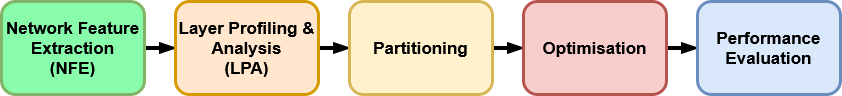
\includegraphics[width=\columnwidth]{Images/Framework.png}
    \caption[CNN Development Flow]{Development flow of Implementing CNNs on Heterogeneous Hardware}
    \label{fig:Framework}
\end{figure}

\subsubsection{Network Feature Extraction \& Layer Profiling Analysis}
Analysing the network architecture is essential in understanding the role of each layer and how they contribute to the overall performance of the model. This is accomplished by running the CNN on various hardware architectures and profiling the execution time and energy consumption of each layer. Once the resource-intensive layers have been identified by profiling, they can be deconstructed into the types of operations they perform. This deconstruction allows for a more granular understanding of the computational requirements.

\subsubsection{Partitioning \& Optimisation}
To efficiently map operations onto hardware, understanding the instruction sets and memory models of different accelerators is necessary. For example, GPUs excel at performing matrix multiplication during high occupancy, while FPGAs are more power and runtime efficient for smaller matrix sizes. CPUs, with their high clock frequency and memory hierarchy, can be advantageous for sequential layers. Optimisations such as quantisation, pruning, and compression can improve performance, but the trade-offs must be carefully considered.

\subsubsection{Performance Evaluation}
 To determine performance, partitioning strategies and hardware choices are benchmarked using various metrics, such as energy consumption, accuracy, inference, and throughput. Evaluating algorithms not only serves as a comparison to other architecture but also identifies areas for improvement.

The following sections, presents an overview of the representative feature extraction and CNN algorithms targeted for partitioning and implementation on heterogeneous platforms. 

\section{Scale-Invariant Feature Transform}
The Scale-Invariant Feature Transform (SIFT) algorithm used to detect and describe local features in images. The SIFT algorithm is designed to be robust to changes in scale, rotation, and partial occlusion. It works in several stages: First, it identifies key points in the image through scale-space extrema detection. These keypoints are then localised more accurately and assigned an orientation. Finally, a descriptor is computed for each keypoint, capturing its local image gradient patterns. These descriptors are used for matching keypoints across different images, making SIFT useful for tasks like object recognition, image stitching, and 3D reconstruction. The in-depth algorithm and its operations are explored in the previous chapter, section \ref{sec:SIFT}.

\subsection{SIFT Algorithm Analysis}

There are several key stages in the SIFT algorithm that vary in computational complexities and hardware implications. This section discusses the complexity, memory footprint and impact of operations on CPU/GPU/FPGA hardware. The full algorithmic description of SIFT is described in Section \ref{sec:SIFT}.   

\subsubsection{Gaussian Pyramid Construction:}
The Gaussian stage of the SIFT algorithm poses a considerable computational load on hardware, not only due to the intensive convolution operations but also because of the memory requirements involved. The process of generating multiple intermediate images, each corresponding to a different scale, can lead to significant memory consumption, particularly for high-resolution images. For a square image with dimensions of N x N, the complexity of the convolution operation grows quadratically with N, resulting in a substantial computational load. This process is repeated for each of the K scales, further adding to the overall computational demand. Moreover, the hardware would require high memory bandwidth for accessing large filter kernels and image matrices. In addition to the computational complexity, the memory footprint of storing multiple Gaussian-filtered images can become a bottleneck, especially when dealing with large images or a high number of scales. Architectures with higher parallelisation and memory caches are more suitable for this stage.

\subsubsection{Extrema Detection:}
The computation required to determine these extrema involves a pixel-by-pixel comparison, evaluating whether each pixel qualifies as an extremum. While this comparison is conducted for every pixel in the image. These are \(O(1)\) operations for each pixel, and given the nature of the operation, lower compute resources are required. The extrema detection algorithm operates independently on each scale level of the pyramid, comparing pixels within a local neighbourhood to identify potential keypoints. Therefore, this stage can be implemented in parallel which maps well to GPUs and FPGAs.

\subsubsection{Orientation and Magnitude Assignment}
While square root and arc tangent operations are less computationally intensive compared to convolutions, they still pose a significant computational burden, especially when performed on a large number of pixels. Hardware support for fixed-point or floating-point arithmetic can significantly accelerate these calculations, as these specialised units are optimised for handling complex mathematical operations.

\subsubsection{Descriptor Generation:}
In the histogram binning and normalization stage of SIFT, local image gradients are quantised into orientation histograms and then normalised to enhance the robustness of feature descriptors. Binning  involves multiplication and addition operations while normalisation involves division which requires more resource logic on hardware. However, the operation intensity is relatively lower than the previous stages which makes it suitable for all architectures.

\subsubsection*{Experimental Design}
The selected profiling times for each stage and on each hardware are shown in \Fig{SIFTAlgoProfiling}. The runtime profiles of each SIFT stage were collected using a robust experimental methodology. The input is a greyscale $3840 \times 2160$ resolution image. The CPU and GPU implementations leveraged the OpenCV SIFT function, while the FPGA was developed using Verilog. The CPU and GPU code is executed 1000 times, and its runtimes are averaged. In the FPGA implementation, the resulting timing graphs from the simulations are used to determine the time taken for each stage. All architectures had 16-bit float precision for their respective designs and algorithms.


\begin{figure}[t]
    \centering
\resizebox{\columnwidth}{!}{\begin{tikzpicture}
  \begin{axis}[                    
  ybar,    
  ymin=0,
  scaled y ticks=false,  
  width=\columnwidth,  
  legend image code/.code={ \draw[#1, draw=none] (0cm,-0.1cm) rectangle (0.5cm,0.3cm);},
  legend style={
    at={(0.77,0.99)},
    anchor=north,
    legend columns=1,
    draw=black,
    fill=white,
    thick
  },
  ylabel={Execution Time (ms)},
  symbolic x coords={Total,Gaussian Pyramid,Extrema Detect,Orientation \& Magnitude,Descriptor Generation},
  xtick=data,
  nodes near coords,
  scaled x ticks=false,
  nodes near coords style={
    font=\tiny,
    anchor=west,
    rotate=90,
    inner xsep=1pt,
    /pgf/number format/.cd,
    fixed,
    precision=5,
    /tikz/every node/.append style={xshift=0.2cm}
  },
  enlarge x limits=0.19,
  bar width=0.6cm,
  x tick label style={
    align=center,   % enable text wrapping
    text width=1.5cm  % set the text width
  }
  ]
  \addplot[pattern=north west lines,pattern color=black, fill=blue!20, postaction={pattern=north east lines}] coordinates {(Total, 896)(Gaussian Pyramid, 684)(Extrema Detect, 112)(Orientation \& Magnitude, 97)(Descriptor Generation, 21)};
  \addplot[pattern=north east lines,pattern color=black,fill=green!40, postaction={pattern=dots}] coordinates {(Total,10)(Gaussian Pyramid, 3)(Extrema Detect, 2)(Orientation \& Magnitude, 4)(Descriptor Generation, 1)};
  \addplot[pattern=dots,pattern color=black,fill=red!30, postaction={pattern=grid}] coordinates {(Total, 12) (Gaussian Pyramid, 6)(Extrema Detect, 3)(Orientation \& Magnitude, 2)(Descriptor Generation,1)};

  \legend{CPU: 5900X,GPU: 3070,FPGA: ZCU106}
  \end{axis}
\end{tikzpicture}
}    
    \caption{{Operation Stage Run-time Profiling: SIFT.}}
    \label{fig:SIFTAlgoProfiling}
\end{figure}

\subsection{SIFT Profiling \& Partitioning Strategy}

\begin{figure}[t]
\centering
  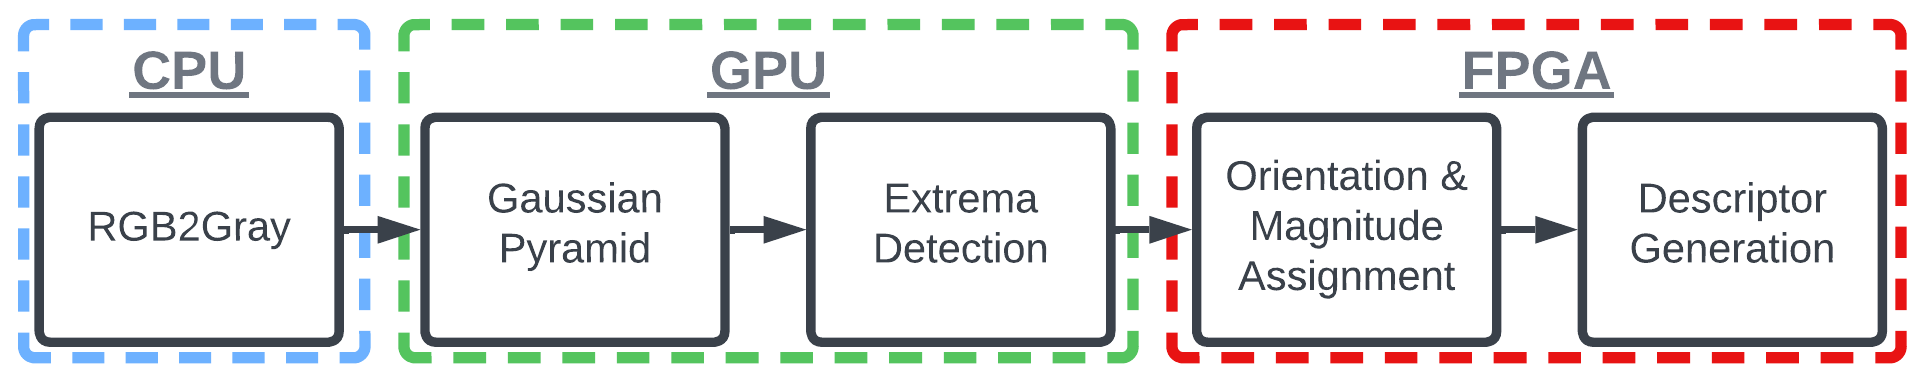
\includegraphics[width=\columnwidth]{Images/SIFT Partition.png}
    \caption{SIFT Algorithm \& Partitioning Strategy.}
    \label{fig:Partitioning}
\end{figure}


The results reveal that the CPU is substantially slower in execution time than GPU and FPGA by $2\times$ on average. Even though the CPU has the highest clock speed, the lack of many processing cores results in poor for-loop unrolling optimisations for parallelisation. Comparing only GPU and FPGA, the overall \textit{Total} runtime has shown the GPU being $0.83 \times$ faster. In the \textit{Gaussian Pyramid} and \textit{Orientation \& Magnitude} stage, the GPU outperforms the FPGA by $2 \times$. On the other hand, the FPGA outperforms the GPU in the \textit{Extrema Detect} stage by $1.5 \times$. The GPU and FPGA architectures are comparable in performance when generating keypoint descriptors due to a lower amount of operations. Overall, the lower GPU runtime in most stages is attributed to having a significantly higher clock speed (\eg 1725MHz vs 300MHz) and more processing cores than the FPGA to maximise throughput.


The partitioning strategy shown in \Fig{Partitioning}, focuses on striking a balance between potential energy consumption and the execution time of the heterogeneous platform.

The RGB to greyscale conversion is a computationally lightweight image processing operation. It involves a linear combination of the red, green, and blue colour channels with specific weightings to produce a greyscale image. The decision to execute \texttt{rgb2gray} algorithm on the CPU instead of the GPU or FPGA is due to minimising the overhead associated with transferring the image data. 
Although GPUs and FPGAs can perform the RGB to Gray conversion slightly faster due to their throughput processing and pipelining capabilities, the time spent moving the data to and from these platforms can negate the benefits, especially for smaller image sizes where the conversion isn't the bottleneck. 

The "\texttt{Gaussian Pyramid}" executed on GPU is faster than the CPU and FPGA since the vast number of cores and memory resources available can utilise majority of the matrix multiplication operations. To create these scale-space representations, the algorithm needs to access the image data repeatedly for each scale level. The Gaussian filters, used to perform blurring, have larger kernels (in terms of memory requirements) as the scale level increases. Additionally, the image data must be read from memory for each scale level, leading to significant memory access. This heavy memory access is due to the repetitive application of convolution operations with Gaussian filters at multiple scales. The memory bandwidth and efficiency become critical in this stage, especially when working with large images or implementing the algorithm on hardware platforms. Therefore, GPUs can provide an advantage in scenarios where larger memory bandwidth is needed over FPGAs. 
The "\texttt{Extrema Detection}" is allocated to GPU to reduce additional data transfer costs that would offset any performance gain. The "\texttt{Orientation \& Magnitude}" operations are better suited to the FPGA due to the customised pipelining offered, which allows a higher number of gradient calculation operations per clock cycle. In the final operation stage, "\texttt{Descriptor Generation}", the FPGA offers comparable performance to the GPU while consuming less energy per operation and reducing additional data transfers.

%-----------------------------------------------------
%  CNN PARTITIONING
%----------------------------------------------------

\section{Convolutional Neural Network}
This section describes the architecture of two widely used CNNs, \textit{Resnet18} and \textit{MobilenetV2}. Each CNN is profiled layer by layer and a partitioning strategy is developed to execute on the heterogeneous platform. The layer characteristics and profiling results support the partitioning methods.

%-----------------------------------------------------
%Partitioning Graph
%-----------------------------------------------------
% \begin{figure}[t]
% \centering
%   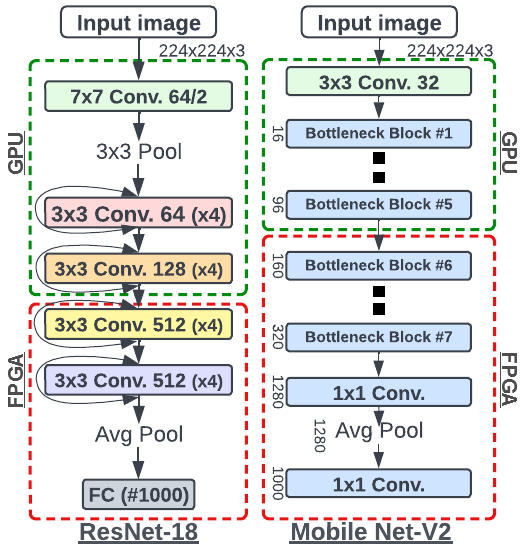
\includegraphics[width=0.8\columnwidth]{Images/RESNET18-4.png}
%     \caption{Resnet18 and MobileNetV2 Architecture \& Partitioning Strategy}
%     \label{fig:CNNArchitectures}
% \end{figure}




% \begin{figure*}[!tb]
%     \centering
%     \begin{tabular}{cc}
%     \resizebox{0.5\linewidth}
%     {!}{\begin{tikzpicture}
  \begin{axis}[                    
  ybar,    
  ymin=0,
  %height=7cm,
  scaled y ticks=false,
  y tick label style={
    /pgf/number format/fixed,
  },
  width=\columnwidth,
  legend image code/.code={
    \draw[#1, draw=none] (0cm,-0.1cm) rectangle (0.5cm,0.3cm);
  },
  legend style={
    at={(0.85,0.99)},
    anchor=north,
    legend columns=1,
    draw=black,
    fill=white,
    thick
  },
  ylabel={Execution Time (s)},
  symbolic x coords={Total,Conv1,L1,L2,L3,L4,FC},
  xtick=data,
  nodes near coords,
  scaled x ticks=false,
  nodes near coords style={
    font=\normalsize,
    anchor=west,
    rotate=90,
    inner xsep=1pt,
    /pgf/number format/.cd,
    fixed,
    precision=5,
    /tikz/every node/.append style={xshift=0.2cm}
  },
  enlarge x limits=0.09,
  bar width=0.4cm,
  ]
  \addplot[pattern=north west lines,pattern color=black, fill=blue!20, postaction={pattern=north east lines}] coordinates {(Total, 0.29)(Conv1, 0.023)(L1, 0.021)(L2, 0.011)(L3, 0.009)(L4, 0.0015)(FC, 0.0001)};

  \addplot[pattern=north east lines,pattern color=black,fill=green!40, postaction={pattern=dots}] coordinates {(Total, 0.18)(Conv1, 0.0025)(L1, 0.0024)(L2, 0.0019)(L3, 0.0019)(L4, 0.0009)(FC, 0.0009)};
  %GPU
  \addplot[pattern=dots,pattern color=black,fill=red!30, postaction={pattern=grid}] coordinates {(Total, 0.19) (Conv1, 0.0034)(L1, 0.0034)(L2, 0.0021)(L3,0.0019)(L4, 0.0009)(FC, 0.0009)};
  %FPGA
  
  \legend{CPU: 5900X,GPU: 3070,FPGA: ZCU102}
  \end{axis}
\end{tikzpicture}
} &
%         \resizebox{0.5\columnwidth}{!}{\begin{tikzpicture}
  \begin{axis}[                      
  ybar,     
  ymin=0,     
  ymax=0.30,
  %height=6.5cm,
  scaled y ticks=false,   
  width=\columnwidth,                                
  legend image code/.code={ \draw[#1, draw=none] (0cm,-0.1cm) rectangle (0.5cm,0.3cm);
  },
  legend style={
    at={(0.85,0.99)},
    anchor=north,
    legend columns=1,
    draw=black,
    fill=white,
    thick
  },
  ylabel={Execution Time (s)},
  symbolic x coords={Total,BN1,BN2,BN3,BN4,BN5,BN6,BN7},
  xtick=data,
  nodes near coords,
  scaled x ticks=false,
  y tick label style={
    /pgf/number format/fixed,
  },
  nodes near coords style={
    font=\normalsize,
    anchor=west,
    rotate=90,
    inner xsep=1pt,
    /pgf/number format/.cd,
    fixed,
    precision=5,
    /tikz/every node/.append style={xshift=0.2cm}
  },
  enlarge x limits=0.09,
  bar width=0.4cm,
  ]
  \addplot[pattern=north west lines,pattern color=black, fill=blue!20, postaction={pattern=north east lines}] coordinates {(Total, 0.241)(BN1,0.02202)(BN2, 0.01502)(BN3, 0.01102)(BN4, 0.00902)(BN5, 0.00802)(BN6, 0.00602)(BN7, 0.00201)};
  
  \addplot[pattern=north east lines,pattern color=black,fill=green!40, postaction={pattern=dots}] 
    coordinates {(Total, 0.23)(BN1, 0.015)(BN2, 0.010)(BN3, 0.007)(BN4, 0.007)(BN5,0.0009)(BN6, 0.0008)(BN7, 0.0008)};
    
  \addplot[pattern=dots,pattern color=black,fill=red!30, postaction={pattern=grid}] coordinates {(Total, 0.20) (BN1, 0.0034)(BN2, 0.0034)(BN3, 0.0021)(BN4, 0.0019)(BN5, 0.001)(BN6, 0.001)(BN7, 0.001)};
  
  \legend{CPU: 5900X,GPU: 3070,FPGA: ZCU102}
  \end{axis}
\end{tikzpicture}
} \\    (a) Resnet18 & (b) MobileNetV2
%     \end{tabular}
%     \caption{Layer Run-time Profiling a) First Convolution (Conv1) Layer (L), Fully Connected (FC) b) Bottleneck Layer (BN) }
%     \label{fig:LayerRuntime}
% \end{figure*}
%========================================

\subsection{Convolution Neural Network Architecture:} 
\begin{figure}[h]
\centering
  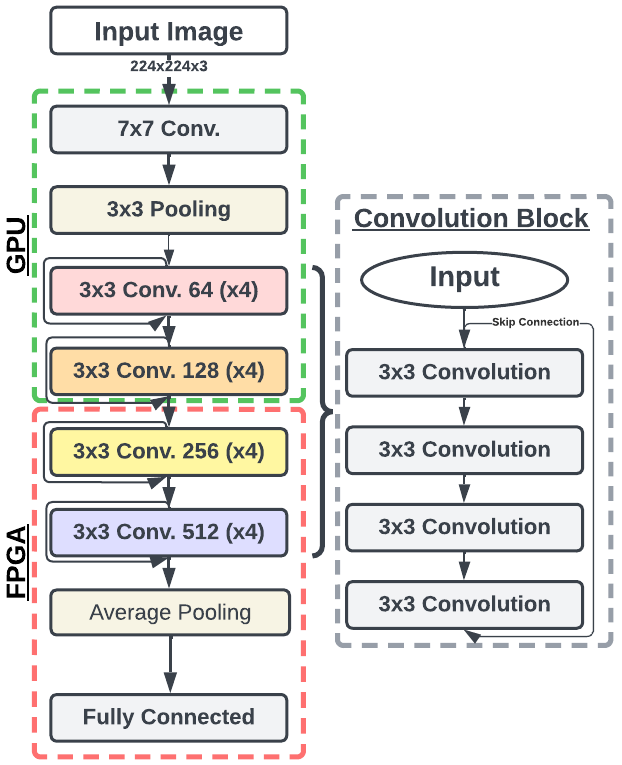
\includegraphics[width=0.6\columnwidth]{Images/Rensnet18.png}
    \caption{ResNet-18 Architecture \& Partitioning Strategy.}
    \label{fig:Rensnet18}
\end{figure}


\textbf{ResNet-18:} is a deep convolutional neural network architecture observed in \ref{fig:Rensnet18}, that employs several key techniques to achieve state-of-the-art performance in various computer vision tasks. Its design is driven by the need to train very deep neural networks while mitigating issues like vanishing gradients. The key components and technical details of ResNet-18 are as follows:



\begin{enumerate}
\item \textbf{Convolutional Layers:} ResNet-18 comprises a total of 18 layers, which are organised into several stages. The first layer is a $7\times7$ convolutional layer with a stride of 2. This layer is followed by a max-pooling operation with a $3\times3$ window and a stride of 2. The large kernel size in the initial layer helps capture larger spatial features.

\item \textbf{Batch Normalisation and ReLU Activation:} After each convolutional layer, batch normalisation is applied to stabilise and accelerate training. This is followed by the Rectified Linear Unit (ReLU) activation function, which introduces non-linearity into the network. The combination of batch normalisation and ReLU helps in faster convergence and regularisation.

\item \textbf{Residual Connections:} One of the distinctive features of ResNet-18 is its use of residual connections. These connections introduce identity mappings, which allow the network to learn the residual information between layers. Mathematically, the output of a residual block is calculated as follows:
\begin{equation}
F(x) = \mathcal{H}(x) + x
\end{equation}
Where \(x\) is the input to the block, \(\mathcal{H}(x)\) represents the transformation applied by the block, and \(F(x)\) is the output.

\item \textbf{Downsampling Blocks:} Each stage in ResNet-18 contains multiple residual blocks. After a series of convolutional layers within a stage, a downsampling block is applied. The downsampling block typically involves a convolutional layer with a stride of 2, which reduces the spatial size of the feature maps while increasing the number of channels. This operation effectively reduces the computational burden while preserving important information.

\item \textbf{Softmax Classification Layer:} The final layer of ResNet-18 is a softmax classification layer. It takes the feature map produced by the preceding layers and computes a probability distribution over output classes. The softmax function is applied to the features, and the resulting probabilities indicate the likelihood of the input belonging to different classes.

\item \textbf{Shortcut Connections:} To prevent vanishing gradients and facilitate the flow of information, shortcut connections are introduced in residual blocks. These connections skip the first two convolutions within a block and add the input directly to the output of the third convolutional layer. This way, the gradient can flow backwards through the skip connection, making it easier to train very deep networks.
\end{enumerate}


% \textbf{ResNet18:} employs batch normalisation and ReLU activation functions after each convolutional layer. The network contains 18 convolutional layers, with the first layer being a $7\times7$ convolutional layer followed by max pooling. ResNet18 also utilises residual connections to learn identity mappings, reducing the impact of vanishing gradients. Each stage contains multiple convolutional layers and is followed by a downsampling block that reduces the spatial size of feature maps while increasing the number of channels. The final output is a softmax classification layer that produces a probability distribution over output classes. Shortcut connections skip the first two convolutions and add the input to the output of the third convolution, avoiding vanishing gradients and improving information flow.

\begin{figure}[h]
\centering
  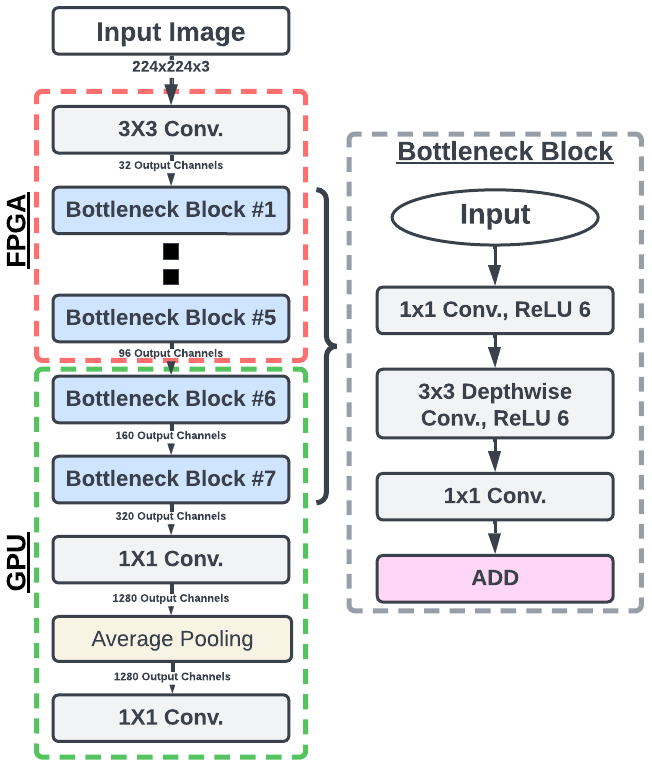
\includegraphics[width=0.6\columnwidth]{Images/MobilnetV2.png}
    \caption{MobileNetV2 Architecture \& Partitioning Strategy.}
    \label{fig:MobileNetV2Architectures}
\end{figure}



\noindent\textbf{MobileNetV2:} shown in \ref{fig:MobileNetV2Architectures}, is an embedded-optimised convolutional neural network architecture that uses a range of techniques to achieve high accuracy with low computational cost. Key details of MobileNetV2 include:
\begin{enumerate}

\item  \textbf{Depthwise Separable Convolution:} MobileNetV2 employs a depthwise separable convolution technique. It divides a standard convolution operation into two distinct steps: depthwise convolution and pointwise convolution. Depthwise convolution first performs a separate convolution for each input channel using a kernel of size $(k, k)$, where $k$ is the filter size. This reduces the computational load by a significant margin.

The depthwise convolution operation is computed using \Eq{depthwise}:
   
\begin{equation}\label{eq:depthwise}
y = \text{depthwise\_conv}(x, W_{d})
\end{equation}
   
where $y$ is the output, $x$ is the input feature map, and $W_{d}$ are the depthwise convolution weights.

\item \textbf{Pointwise Convolution:} After the depthwise convolution, pointwise convolution is applied using $1\times1$ kernels. Pointwise convolution combines the results of the depthwise convolution by performing a linear combination of the channels. This step helps to capture complex relationships between channels and is critical for maintaining model accuracy.

The pointwise convolution operation shown in  ~\Eq{Pointwise}:
   
\begin{equation}\label{eq:Pointwise}
y = \text{pointwise\_conv}(x, W_{p})
\end{equation}

where $y$ is the output, $x$ is the result of the depthwise convolution, and $W_{p}$ are the pointwise convolution weights.

\item \textbf{Reduction of Computational Cost and Parameters:} The combination of depthwise separable convolution reduces the computational cost significantly, making MobileNetV2 suitable for resource-constrained embedded devices. The reduction in the number of parameters and the computational requirements is a crucial advantage.

\item \textbf{Linear Bottlenecks:} MobileNetV2 also introduces linear bottlenecks, which are inexpensive $1\times1$ convolutions placed between a ReLU activation function and a $3\times3$ convolution. These linear bottlenecks are designed to keep the computational cost low while ensuring that the network maintains a high level of accuracy. The ReLU activation helps introduce non-linearity, while the subsequent $3\times3$ convolution captures more complex features.

 The linear bottleneck operation represented in ~\Eq{bottleneck}:
   
\begin{equation}\label{eq:bottleneck}
y = \text{conv\_3x3}(\text{ReLU}(\text{conv\_1x1}(x, W_{l})), W_{3x3})
\end{equation}
   
   where $y$ is the output, $x$ is the input, $W_{l}$ are the linear bottleneck weights, and $W_{3x3}$ are the weights for the $3\times3$ convolution.
\end{enumerate}





\subsection{CNN Profiling \& Partitioning Strategy:} 
%----------------------------------------------------------PROFILING GRAPHS
%---------------------------------------------------------
%
\begin{figure}[tb]
    \centering
\resizebox{\columnwidth}{!}{\begin{tikzpicture}
  \begin{axis}[                    
  ybar,    
  ymin=0,
  %height=7cm,
  scaled y ticks=false,
  y tick label style={
    /pgf/number format/fixed,
  },
  width=\columnwidth,
  legend image code/.code={
    \draw[#1, draw=none] (0cm,-0.1cm) rectangle (0.5cm,0.3cm);
  },
  legend style={
    at={(0.85,0.99)},
    anchor=north,
    legend columns=1,
    draw=black,
    fill=white,
    thick
  },
  ylabel={Execution Time (s)},
  symbolic x coords={Total,Conv1,L1,L2,L3,L4,FC},
  xtick=data,
  nodes near coords,
  scaled x ticks=false,
  nodes near coords style={
    font=\normalsize,
    anchor=west,
    rotate=90,
    inner xsep=1pt,
    /pgf/number format/.cd,
    fixed,
    precision=5,
    /tikz/every node/.append style={xshift=0.2cm}
  },
  enlarge x limits=0.09,
  bar width=0.4cm,
  ]
  \addplot[pattern=north west lines,pattern color=black, fill=blue!20, postaction={pattern=north east lines}] coordinates {(Total, 0.29)(Conv1, 0.023)(L1, 0.021)(L2, 0.011)(L3, 0.009)(L4, 0.0015)(FC, 0.0001)};

  \addplot[pattern=north east lines,pattern color=black,fill=green!40, postaction={pattern=dots}] coordinates {(Total, 0.18)(Conv1, 0.0025)(L1, 0.0024)(L2, 0.0019)(L3, 0.0019)(L4, 0.0009)(FC, 0.0009)};
  %GPU
  \addplot[pattern=dots,pattern color=black,fill=red!30, postaction={pattern=grid}] coordinates {(Total, 0.19) (Conv1, 0.0034)(L1, 0.0034)(L2, 0.0021)(L3,0.0019)(L4, 0.0009)(FC, 0.0009)};
  %FPGA
  
  \legend{CPU: 5900X,GPU: 3070,FPGA: ZCU102}
  \end{axis}
\end{tikzpicture}
}    %\caption{Execution times for individual and combined algorithms.}
    %\vspace{-6mm}
    \caption[ResNet18 Layer Profiling]{{ResNet18, Layer Run-time Profiling: First Convolution (Conv1) Layer (L), Fully Connected (FC). Total represents the complete CNN running including initialisation time.}}
    \label{fig:Resnet18LayerRuntime}
\end{figure}



%Algorithm profiling is an important step in determining the best processor for efficient execution. It involves measuring and analysing the performance of the individual operations within the algorithm, with the goal of identifying any bottlenecks or inefficiencies that may be impacting system performance. In partitioning 

In this section, both CNN architectures are analysed and partitioned onto the appropriate accelerator based on their runtime profiles. The CNN hardware comparison results are displayed in Figure \Fig{Resnet18LayerRuntime} \& \Fig{MobilenetLayerRuntime}.

\subsubsection*{Experimental Design}
The runtime profiles of each CNN architecture layer were collected using a robust experimental design. Both MobileNetV2 and ResNet18 architectures used a $3840 \times 2160$ resolution image dataset. The CPU and GPU implementations leveraged the Pytorch library and its CUDA configuration. A custom hook function was defined to measure the runtime of each convolutional and linear layer during forward pass execution. For every convolutional and linear layer in the model, the hook function recorded the start and end times, allowing calculation of the layer-wise runtime. Through 1000 code execution iterations, the runtimes collected are averaged. In the FPGA implementation, Xilinx deep learning processing unit IP and their resulting timing graphs are used to determine the time taken by each layer. All architectures had 8-bit precision for both models and implementation.



\subsubsection{\textbf{Resnet18:}}
The \textit{Resnet18} results in \Fig{Resnet18LayerRuntime} show the fastest hardware for executing the model is the GPU, with the total execution time of $0.18$s, while the slowest is the CPU with $0.29$s. The FPGA's total execution time is between the two with $0.19$s.

The \texttt{conv1} layer is computationally intensive for all 
platforms as it applies 64 filters of size $7\times7$ to a large input image with multiple colour channels. This results in a large number of multiply-accumulate (MAC) operations. The conv1 layer also performs padding and activation functions, which adds to the overall computational cost. However, the execution time for Conv1 is significantly faster on the GPU, which can parallelise the computations across multiple cores. In layers $L1\sim L2$, the GPU is $1.36\times$ and $1.10\times$ faster than the FPGA. Therefore, the GPU is the best candidate to allocate Conv1, L1 and L2 for execution. 

The $L3\sim L4$ and Fully Connected (FC) layers take relatively less time to execute. The size of feature maps decreases as they progress through the layers due to downsampling operations like pooling and strides. The $L3\sim L4$ convolutional and average pool layers can be executed on the FPGA since fewer MAC operations are occurring for the GPU to be fully utilised while taking advantage of power efficient architecture. 


\begin{figure}[tb]
    \centering
\resizebox{\columnwidth}{!}{\begin{tikzpicture}
  \begin{axis}[                      
  ybar,     
  ymin=0,     
  ymax=0.30,
  %height=6.5cm,
  scaled y ticks=false,   
  width=\columnwidth,                                
  legend image code/.code={ \draw[#1, draw=none] (0cm,-0.1cm) rectangle (0.5cm,0.3cm);
  },
  legend style={
    at={(0.85,0.99)},
    anchor=north,
    legend columns=1,
    draw=black,
    fill=white,
    thick
  },
  ylabel={Execution Time (s)},
  symbolic x coords={Total,BN1,BN2,BN3,BN4,BN5,BN6,BN7},
  xtick=data,
  nodes near coords,
  scaled x ticks=false,
  y tick label style={
    /pgf/number format/fixed,
  },
  nodes near coords style={
    font=\normalsize,
    anchor=west,
    rotate=90,
    inner xsep=1pt,
    /pgf/number format/.cd,
    fixed,
    precision=5,
    /tikz/every node/.append style={xshift=0.2cm}
  },
  enlarge x limits=0.09,
  bar width=0.4cm,
  ]
  \addplot[pattern=north west lines,pattern color=black, fill=blue!20, postaction={pattern=north east lines}] coordinates {(Total, 0.241)(BN1,0.02202)(BN2, 0.01502)(BN3, 0.01102)(BN4, 0.00902)(BN5, 0.00802)(BN6, 0.00602)(BN7, 0.00201)};
  
  \addplot[pattern=north east lines,pattern color=black,fill=green!40, postaction={pattern=dots}] 
    coordinates {(Total, 0.23)(BN1, 0.015)(BN2, 0.010)(BN3, 0.007)(BN4, 0.007)(BN5,0.0009)(BN6, 0.0008)(BN7, 0.0008)};
    
  \addplot[pattern=dots,pattern color=black,fill=red!30, postaction={pattern=grid}] coordinates {(Total, 0.20) (BN1, 0.0034)(BN2, 0.0034)(BN3, 0.0021)(BN4, 0.0019)(BN5, 0.001)(BN6, 0.001)(BN7, 0.001)};
  
  \legend{CPU: 5900X,GPU: 3070,FPGA: ZCU102}
  \end{axis}
\end{tikzpicture}
}    %\caption{Execution times for individual and combined algorithms.}
    %\vspace{-6mm}
    \caption[MobileNetV2, Layer Profiling]{MobileNetV2 Layer Run-time Profiling: Bottleneck Layer (BN). Total represents the complete CNN running including initialisation time.}
    \label{fig:MobilenetLayerRuntime}
\end{figure}

\subsubsection{\textbf{MobilenetV2:}}
The \Fig{MobilenetLayerRuntime} results show that the total execution time for the CNN on the CPU was $0.241$s, while on the GPU and the FPGA, it was $0.23$s and $0.20$s, respectively. The bottleneck layer with the longest execution time for all three devices was BN1, with a time of $0.02202$ms on the CPU, $0.015$ms on the 3070 GPU, and $0.0034$ms on the FPGA.


The runtime for each bottleneck layer decreases as it moves from \texttt{Bottleneck 1} to \texttt{Bottleneck 7} due to reduced input channels and the amount of computation required to process the data in each layer. Thus, the later bottleneck layers take less time to execute than the earlier ones. The first five bottleneck layers are suitable for execution on the FPGA, as it shows that it performs $\sim4\times$ faster than the GPU on average. The reason behind the faster execution on FPGA can attributed to multiple factors below:
\begin{enumerate}
    \item Direct, custom and optimised routing between logic allows efficient data-flow transfer and locality.
    \item Separable filters and feature maps have reduced memory footprint which can be efficiently managed.
    \item Efficient use of pipelining for convolutional operations and reduced data dependency (\eg ResNet18 residual connections).
\end{enumerate}

The remaining \texttt{Bottleneck 5 $\sim 7$} layers are suitable for execution on the GPU because of a slight performance advantage and shorter initialisation transfer time back to the host. The \texttt{Softmax} and \texttt{fully connected} layers are also computed on the GPU since the performance is comparable to the FPGA and reduces data transfer overhead. Both layers are required to transform features into a suitable format, and it assigns a probability score for classification. 

%Although, the later bottleneck layers have less computations, but still require more complex computations, such as convolutions or pooling operations with large windows, which can be efficiently implemented on the FPGA's. Dividing the computation load between the GPU and the FPGA, the overall execution time of the network can be reduced, improving performance.

%The first five bottleneck layers are suitable to be executed on the GPU due to their high parallel computation requirements. However, the last two bottleneck layers are better suited for the FPGA due to less operations but still require complex computations such as convolutions or pooling operations with large windows. Dividing the computation load between the GPU and the FPGA, the overall execution time of the network can be reduced, leading to improved performance.

\section{Experimental Setup}
This section introduces both heterogeneous implementations and their corresponding tools and software used to target those architectures. In addition, a detailed break of the scheduler used to move data between all accelerators while keeping tasks synchronised. Both power and execution time are discussed in detail which are used to evaluate both platforms.The proposed partitioning is tested using two developed heterogeneous platforms containing high-low power components, as shown in Table \ref{tab:HWEnvironment}, and described below:

\begin{table}[tb]
\centering
\setlength{\extrarowheight}{0pt}
\addtolength{\extrarowheight}{\aboverulesep}
\addtolength{\extrarowheight}{\belowrulesep}
\setlength{\aboverulesep}{0pt}
\setlength{\belowrulesep}{0pt}
\caption{Hardware/Software Environment}
\label{tab:HWEnvironment}
\resizebox{\linewidth}{!}{%
\begin{tabular}{c|c|c|c} 
\toprule
\rowcolor[rgb]{0.753,0.753,0.753} \textbf{Accelerator} & \textbf{High-Power} & \textbf{Low-Power} & \textbf{Software} \\ 
\midrule
CPU & \begin{tabular}[c]{@{}c@{}}AMD 5900x \\ (4.8 GHz)\end{tabular} & \begin{tabular}[c]{@{}c@{}}ARMv8.2 \\ (1400MHz)\end{tabular} & Python / Pytorch 2.0 \\ 
\midrule
GPU & \begin{tabular}[c]{@{}c@{}}Nvidia 3070 \\ (1730 MHz)\end{tabular} & \begin{tabular}[c]{@{}c@{}}Xavier NX \\ (1100MHz)\end{tabular} & Python / Pytorch 2.0 \\ 
\midrule
FPGA & \begin{tabular}[c]{@{}c@{}}ZCU106 \\ (300Mhz)\end{tabular} & \begin{tabular}[c]{@{}c@{}}Artix-7 \\ (100MHz)\end{tabular} & Verilog / Vivado / Vitis \\
\bottomrule
\end{tabular}
}
\end{table} 


% \begin{figure}[H]
%     \centering
%     \begin{tabular}{cc}
%     \resizebox{0.48\linewidth}{!}{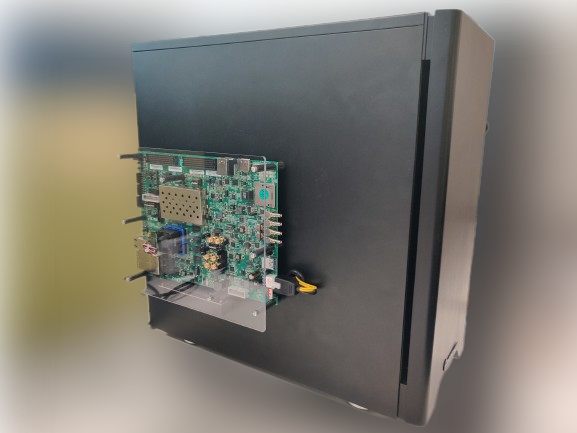
\includegraphics{Images/blurredhp.png}} &
%     \resizebox{0.48\linewidth}{!}{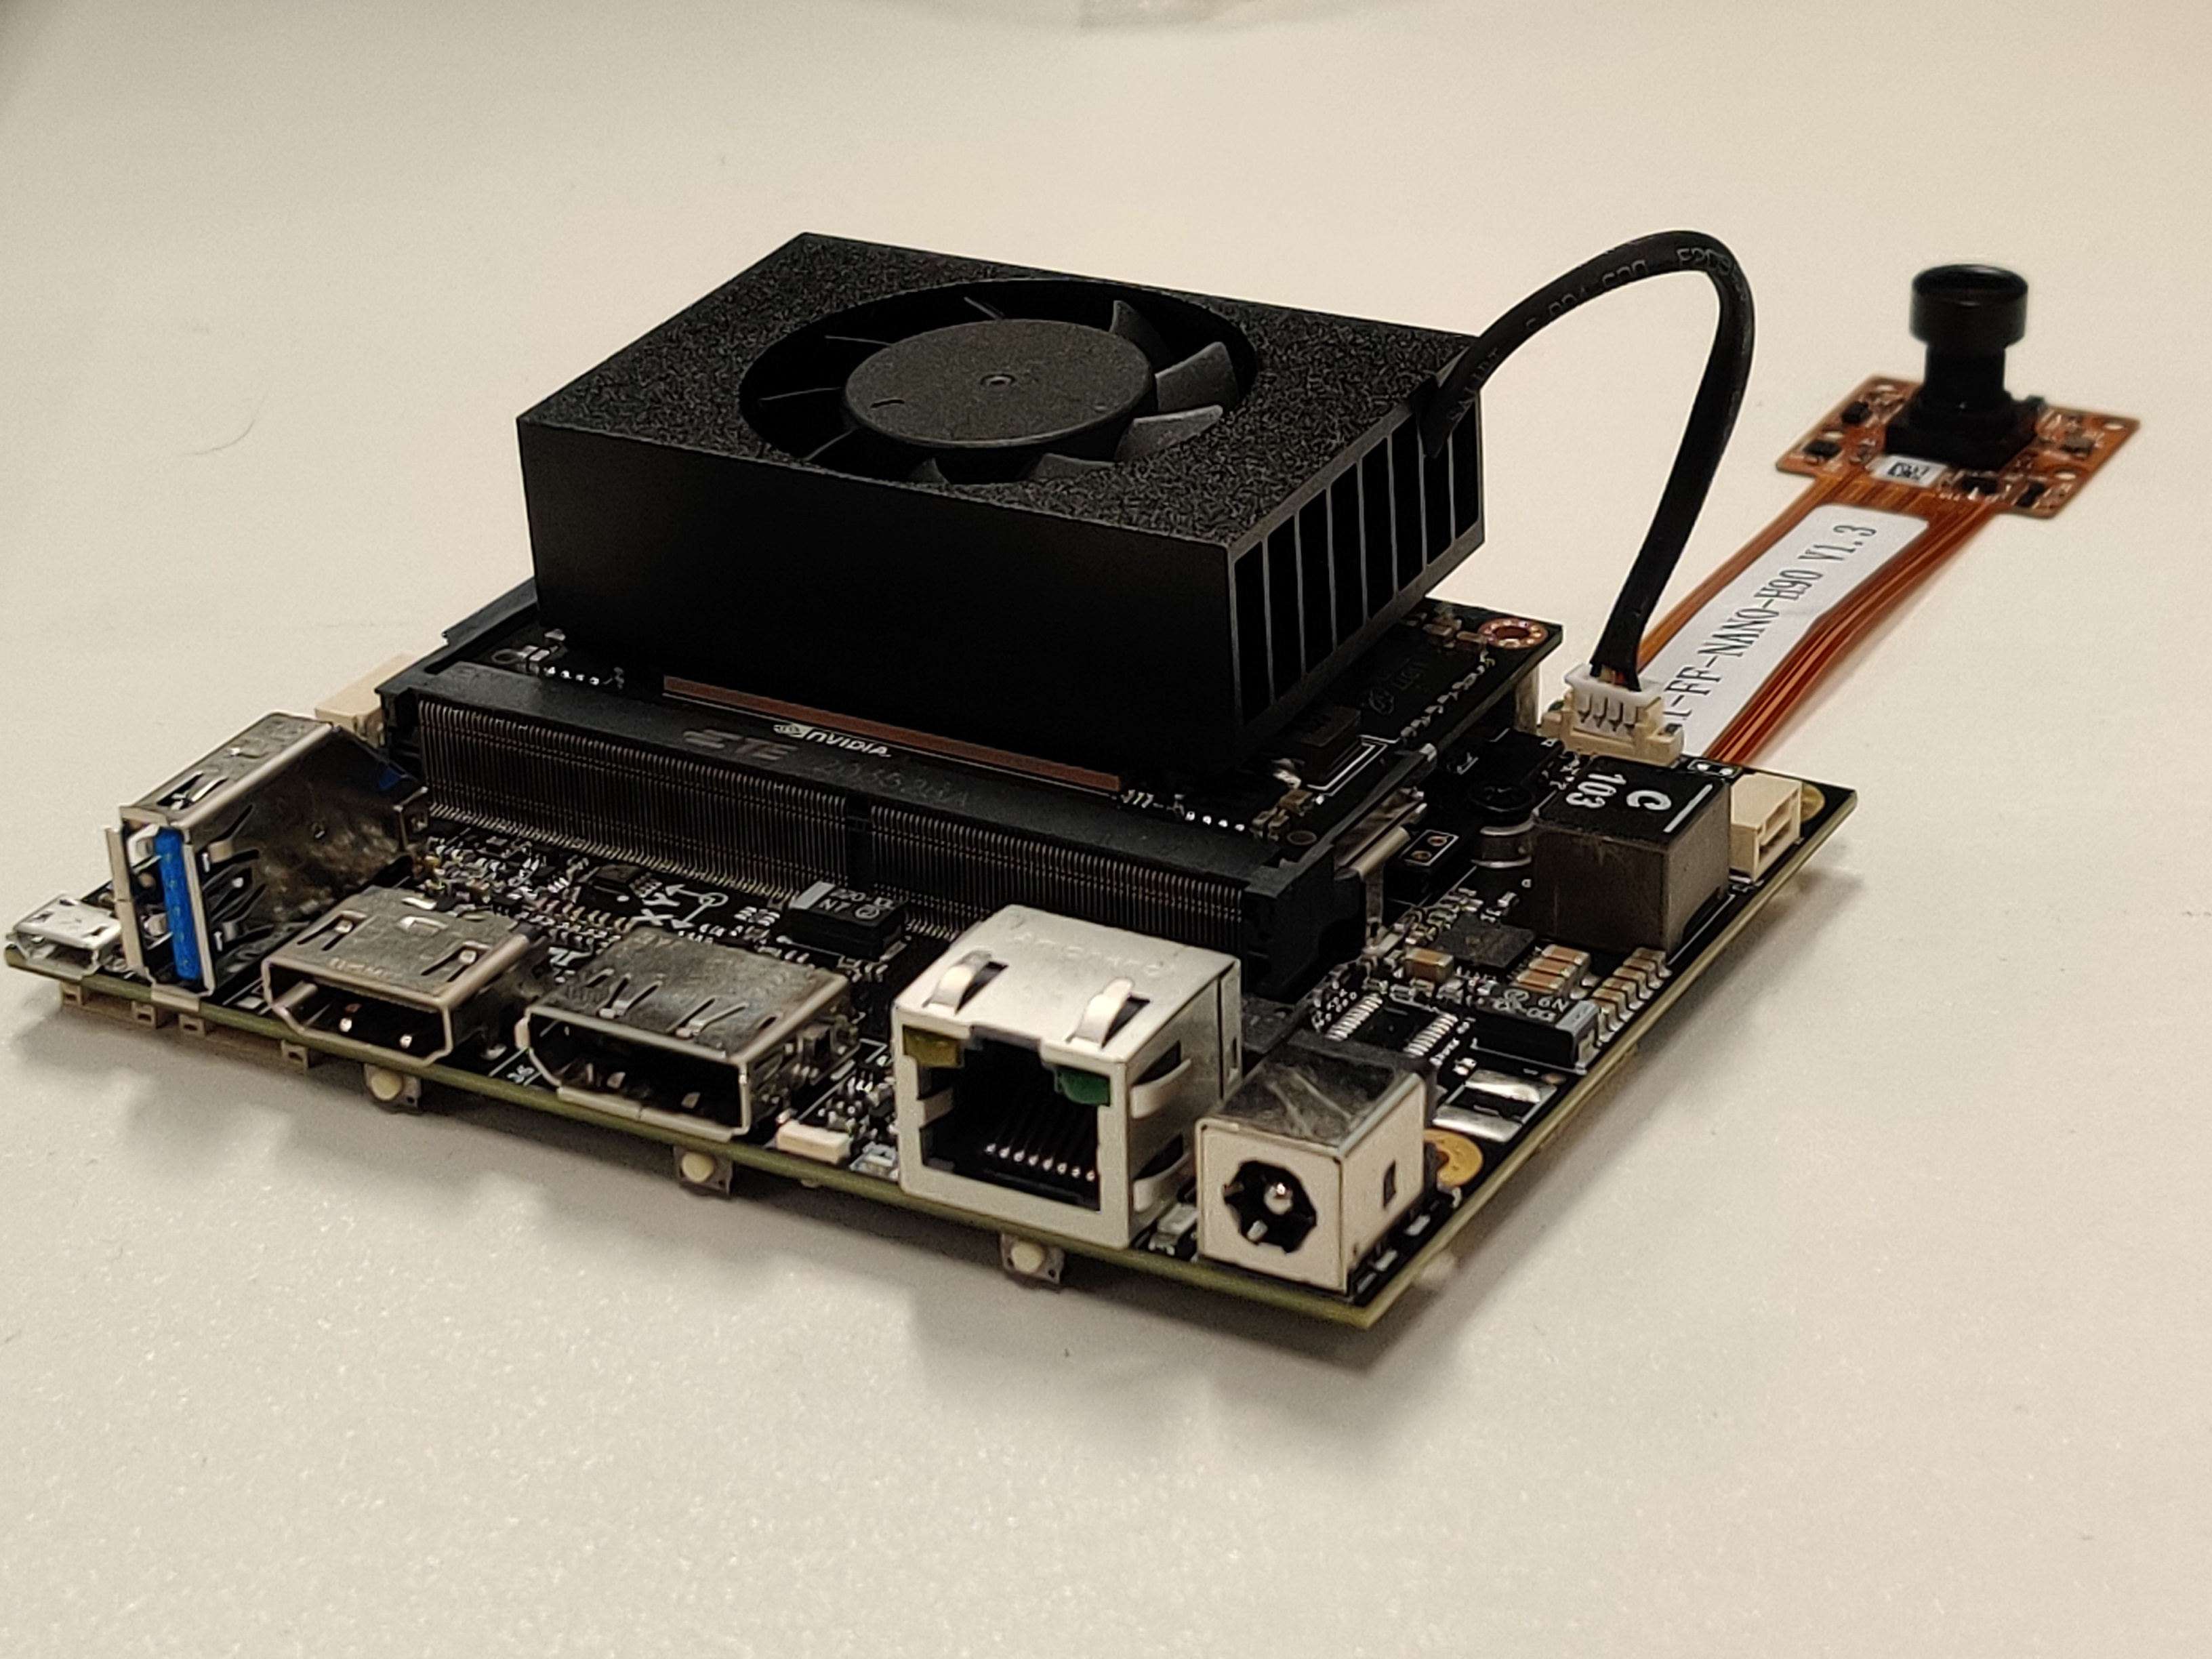
\includegraphics{Images/IMG_20221018_143611.jpg}} \\
%     (a) & (b) \\
%     \end{tabular}
%     \caption[Heterogeneous Platforms]{Heterogeneous Low-Power Embedded System (left) and High-Power System (right) }
%     \label{fig:Clamp}
% \end{figure}
\begin{figure}[tb]
    \centering
    \begin{tabular}{cccc}
        \resizebox{0.48\linewidth}{!}{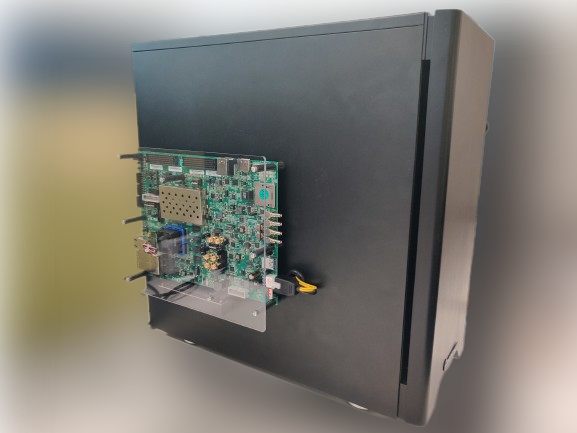
\includegraphics{Images/blurredhp.png}} &
        \resizebox{0.48\linewidth}{!}{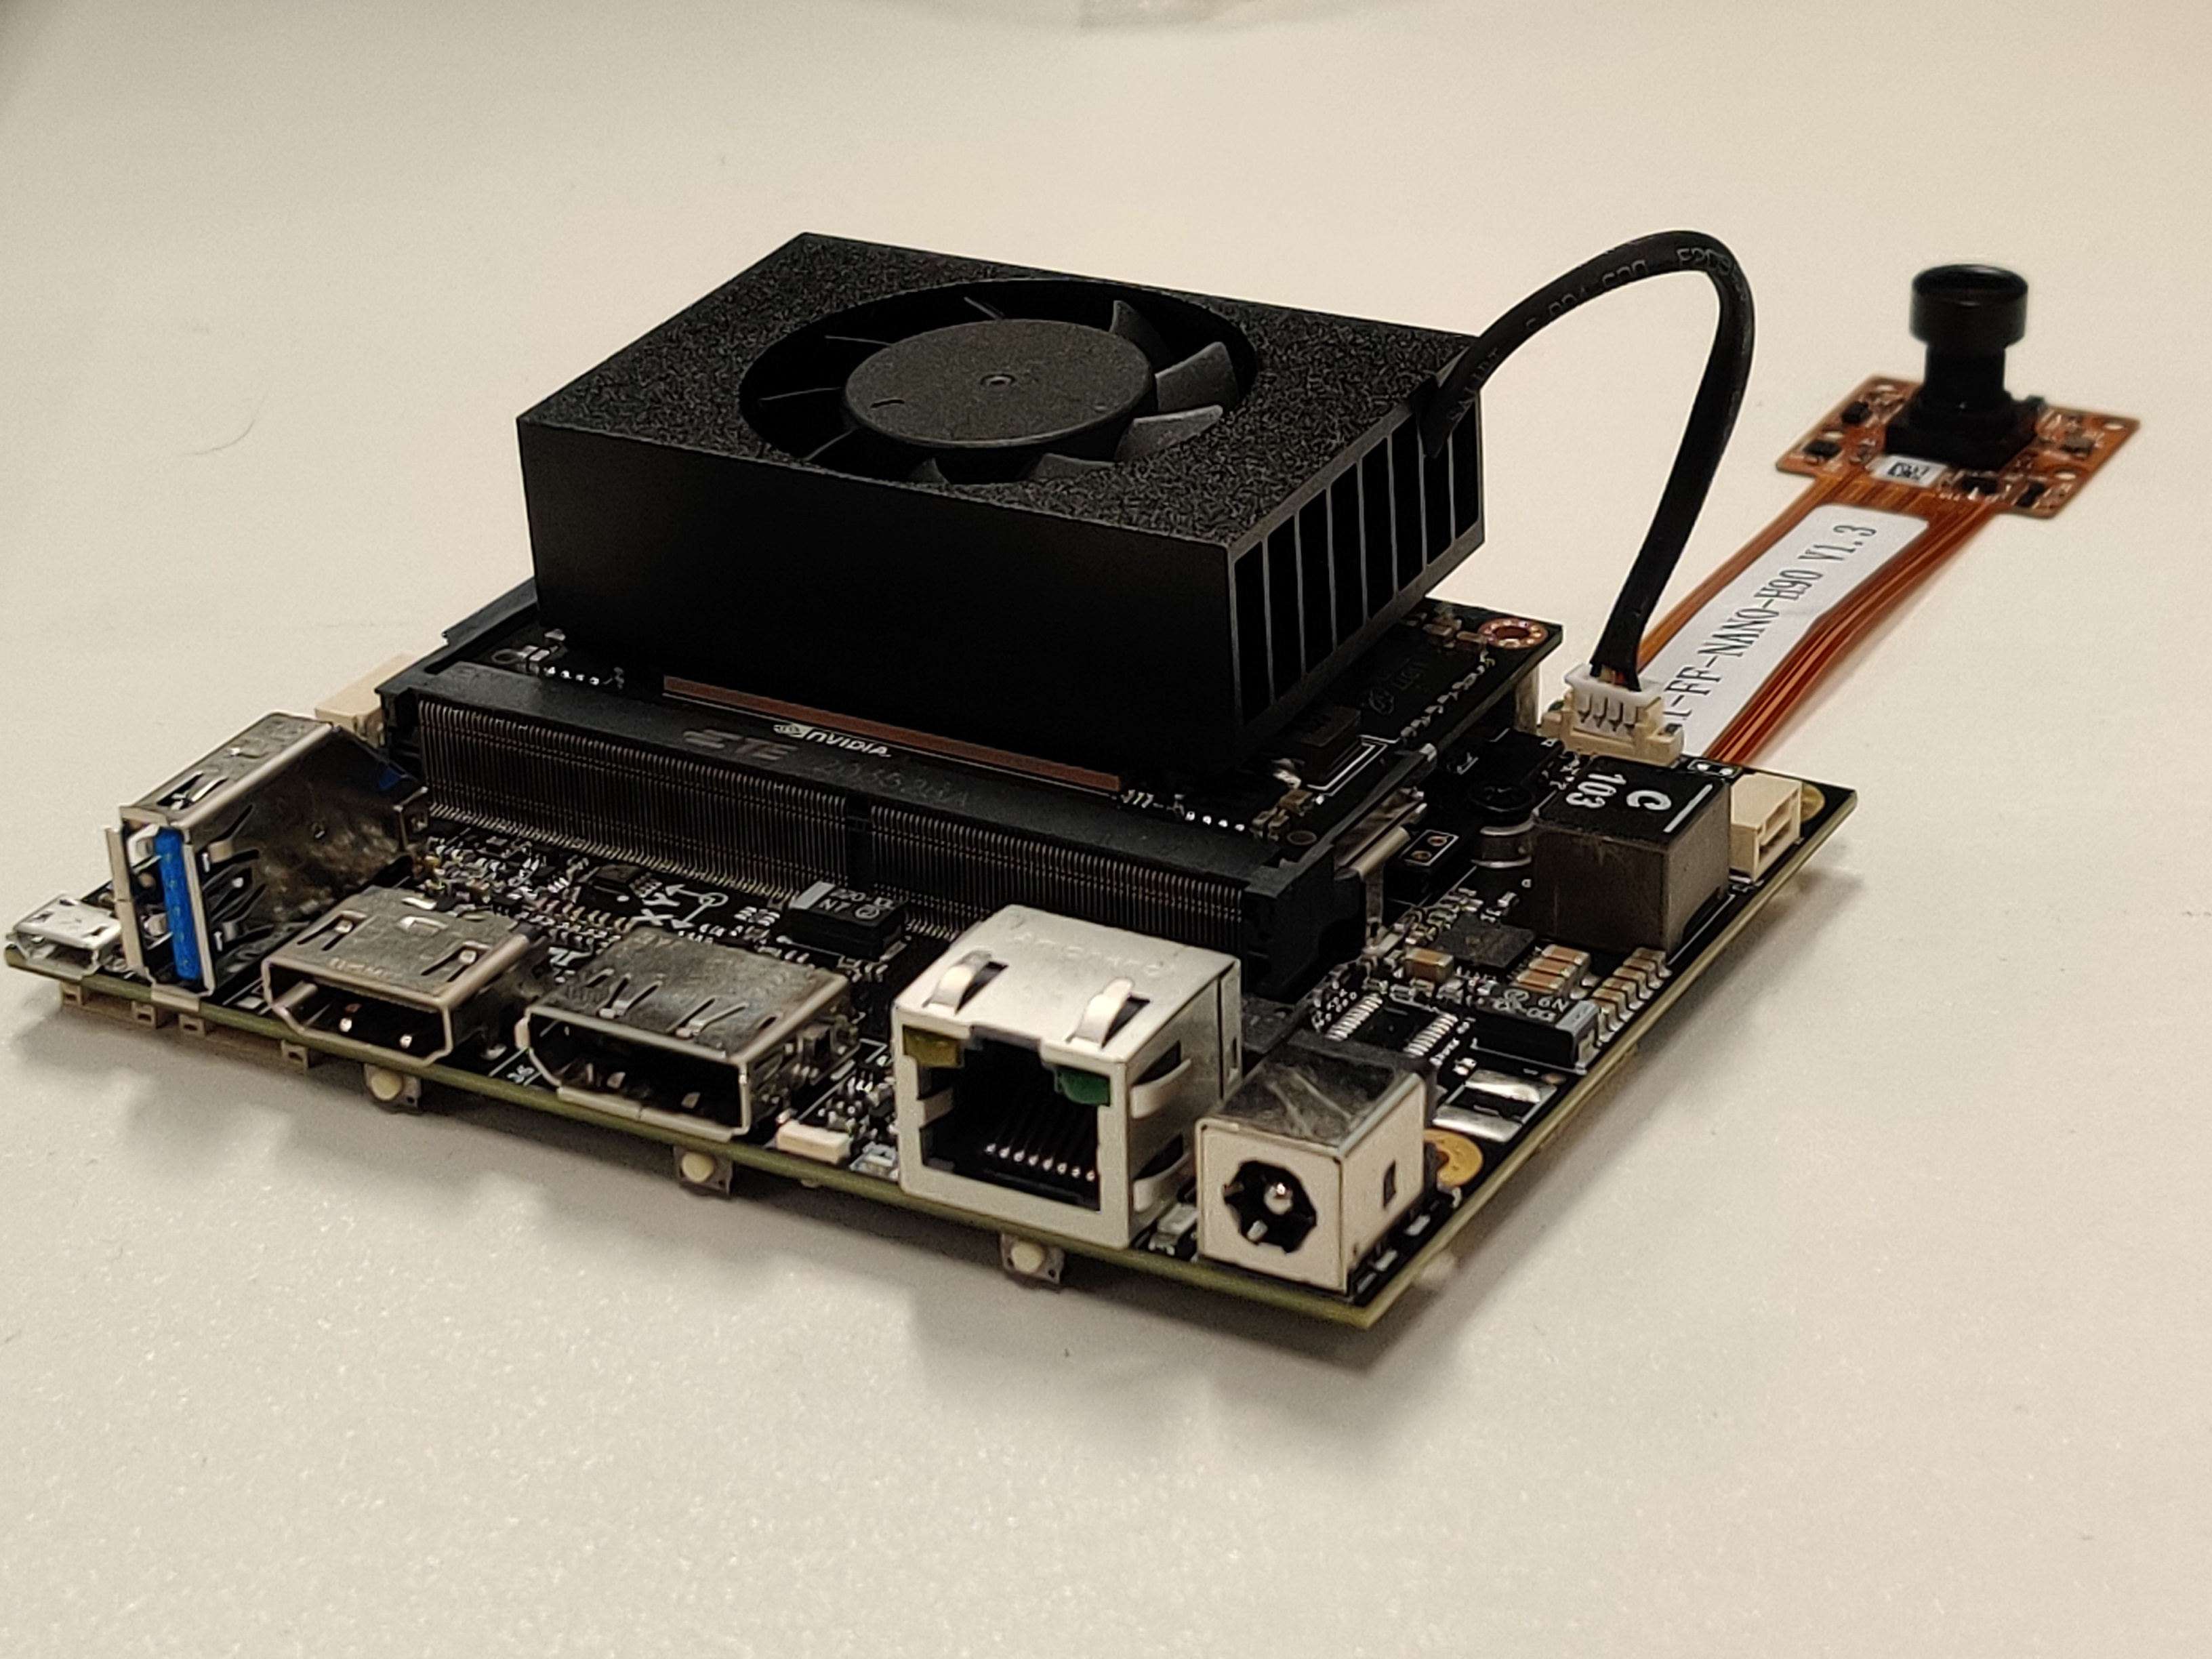
\includegraphics{Images/IMG_20221018_143611.jpg}} \\
        \\
        \resizebox{0.48\linewidth}{!}{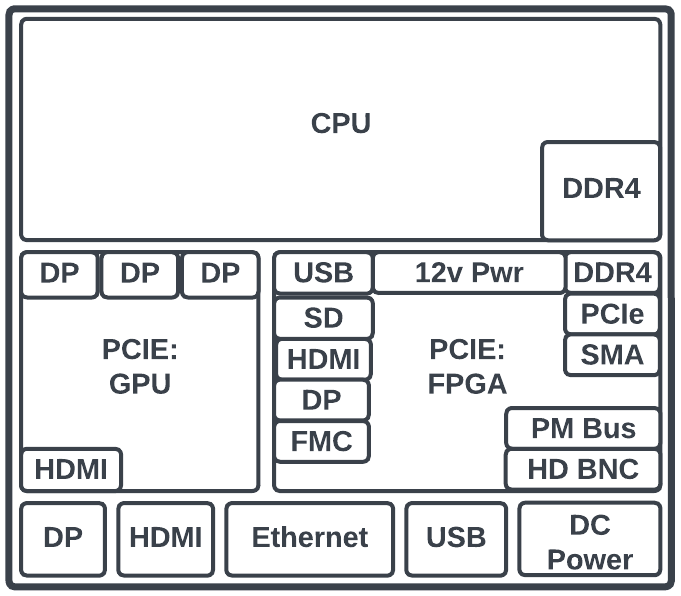
\includegraphics{Images/High Power.png}} &
        \resizebox{0.48\linewidth}{!}{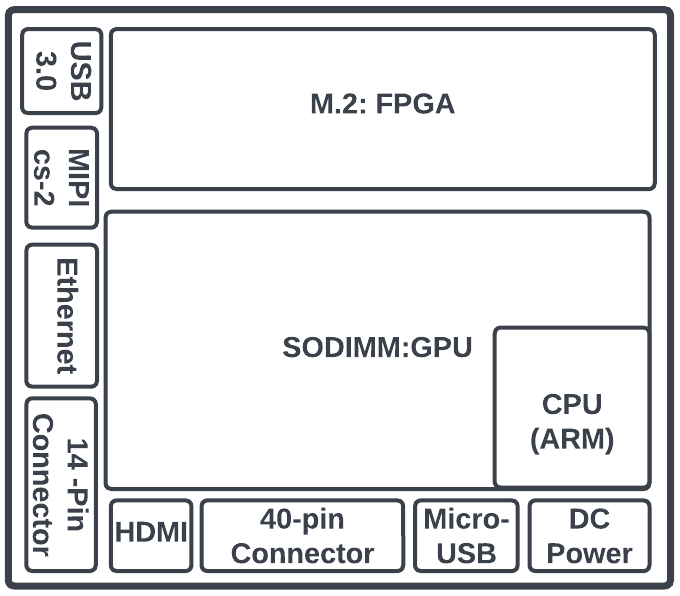
\includegraphics{Images/Low-Power.png}} \\
        (a) & (b) \\
    \end{tabular}
    \caption[Heterogeneous Platforms]{(a) Heterogeneous High-Power System, (b) Low-Power Embedded System}
    \label{fig:Clamp}
\end{figure}


\textbf{Low-Power System:}
The constructed system consists of a custom carrier board which is equipped with several key components, including an Artix-7 (XC7A200T) FPGA, a Jetson Xavier NX, and an ARM CPU. To provide additional storage space, the Linux image is flashed onto the SD card rather than the 16Gb eMMC. Communication between the FPGA and the Xavier NX is achieved through a PCIe gen2 4-lane interface, which is connected via an M.2 key-M connector.  

\textbf{High-Power System:}
The system consists of  CPU (AMD 5900x), GPU (GTX 3070) and FPGA (Xilinx ZCU106), integrated into a desktop with 32GB 3200Mhz DDR4 Memory. Both devices are interfaced via PCIe Gen3 and the communication to the host CPU uses direct memory access (DMA), allowing the movement of data between host memory and subsystems. The GPU and FPGA drivers are used to program the DMA engine and DMA/bridge subsystem IP. Idle CPU is frequency scaled to reduce power consumption. 

\textbf{Dataset.} The test images used in the experiments are from LIU4K-v2 dataset \cite{LiuliuYan19}, which is a high resolution data-set that includes 2000 $3840\times2160$ images. The images contain a variety of backgrounds and objects. 

\subsection*{Heterogeneous Scheduler Architecture}
\begin{figure}[tb]
\centering
 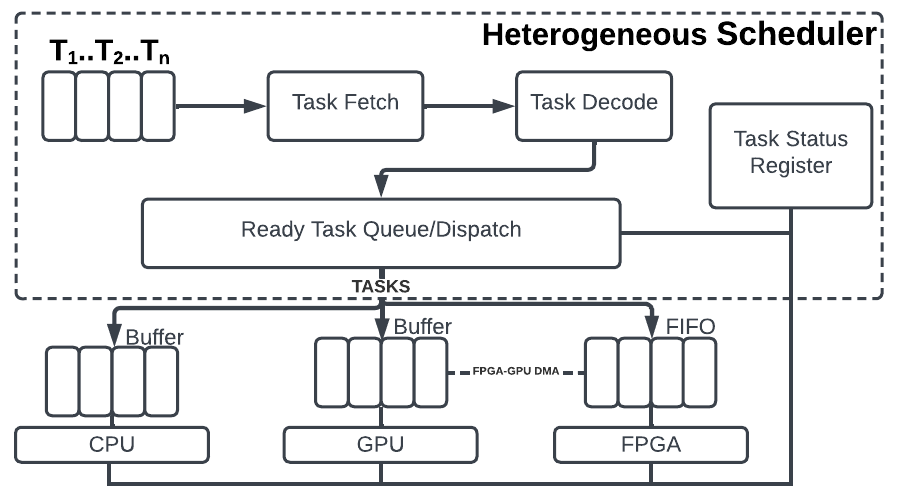
\includegraphics[width=\columnwidth]{Images/SchedulerDetail.png}
   \caption[Scheduler Architecture]{Scheduler Architecture for Heterogeneous Platform: Allocating tasks to processors depending on the partitioning strategy.}
   \label{fig:SchedulerArch}
\end{figure}
A heterogeneous scheduler architecture in \Fig{SchedulerArch} is developed, which is responsible for distributing and managing tasks or workloads across different types of processing units or resources. The scheduler is written in C/C++ to manage memory transfers and pass the feature map and operation stage data from the CPU and into the GPU or FPGA.

The scheduler uses a \textit{First-Come, First-Served} (FCFS) algorithm due to its relatively simple construction and minimal runtime overhead. The operation stages in imaging algorithms are executed sequentially. Therefore, tasks are partitioned in order based on their dependency on previous task data, which makes it suitable for this type of scheduling algorithm. The pre-partitioned ordered tasks are fetched from the queue and decoded to prepare for execution. As tasks are dequeued, they are placed in the task ready queue, a staging area where tasks await execution. The task ready queue ensures that tasks are readily available for the execution stage. Each task contains a predefined pragma which tells the scheduler which architecture to execute the operation on. Additionally, a task status register is used to keep track of the current state and progress of each task. This register provides real-time information about the task's status, whether it is waiting, executing, or completed. The task status register is essential for maintaining task synchronisation and ensuring that tasks progress through the execution pipeline smoothly. It allows the scheduler to monitor and manage the execution of tasks and make informed decisions based on the tasks' statuses, ensuring optimal resource utilisation and order of execution.


\begin{algorithm}[tb]
\caption{Heterogeneous Scheduler}
\label{Alg:HeterogeneousScheduler}
\begin{algorithmic}[1]
    \State $fpga\_output \gets \text{None}$
    \State $gpu\_output \gets \text{None}$
    \State $task\_queue \gets \emptyset$  \Comment{FCFS task queue}
    
    \For{$i \gets 1$ to $\text{Length}(tasks)$}
        \State $task \gets \text{tasks}[i]$
        \State $task\_queue \gets task\_queue \cup \{task\}$  \Comment{Add task to FCFS queue}
    \EndFor

    \While{$task\_queue$ is not empty}
        \State $task \gets \text{Dequeue}(task\_queue)$  \Comment{Dequeue the first task}
        
        \If{$\text{ExecuteOnFPGA}(task, fpga\_partition)$}
            \State $fpga\_output \gets \text{ExecuteOnFPGA}(task)$
        \ElsIf{$\text{ExecuteOnGPU}(task, gpu\_partition)$}
            \State $gpu\_output \gets \text{ExecuteOnGPU}(task)$
        \EndIf
    \EndWhile
    
    \If{$fpga\_output$ is not \text{None}}
        \State $final\_output \gets \text{TransferData}(fpga\_output, "FPGA", "CPU")$
    \Else
        \State $final\_output \gets \text{TransferData}(gpu\_output, "GPU", "CPU")$
    \EndIf
    
    \State $final\_output \gets \text{PostProcess}(final\_output)$
    \State $\text{DisplayResult}(final\_output)$
\end{algorithmic}
\end{algorithm}


The pseudocode presented in Algorithm~\ref{Alg:HeterogeneousScheduler} outlines the process of the Heterogeneous Scheduler. This algorithm iterates over the tasks in the workload and employs an FCFS queue to execute tasks in the order they were received. The algorithm initialises two functions, \texttt{ExecuteOnFPGA()} and \texttt{ExecuteOnGPU()}, which are used to execute the task on a certain device based on a partitioning strategy. The FCFS queue ensures that tasks are executed in the order of arrival, maintaining fairness and accuracy in task execution. Once all tasks have been executed, the algorithm transfers the output data from the FPGA or GPU to the CPU, depending on which device the output is stored on. This transfer facilitates the consolidation of results for further processing. Lastly, the algorithm post-processes the output to generate the final result of the workload. 



\subsection{CPU-GPU-FPGA Data Communication}

\begin{figure}[tb]
\centering
 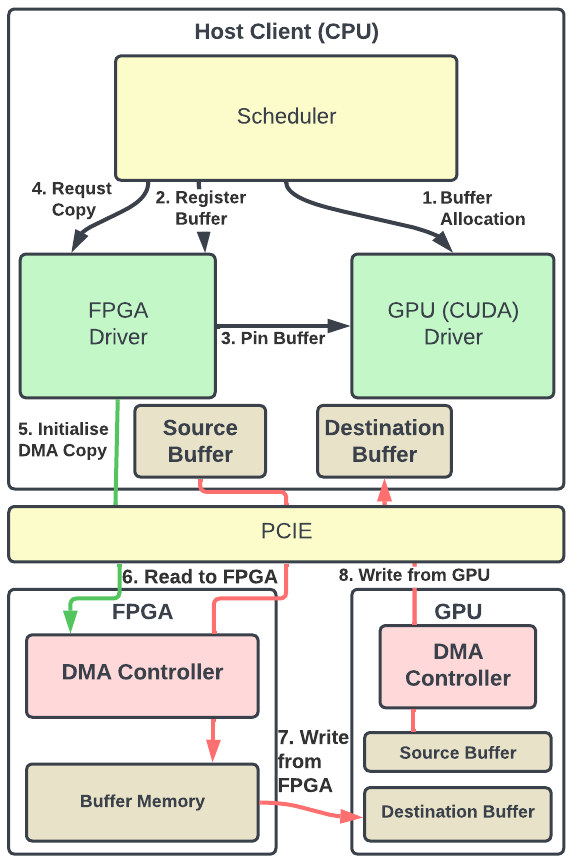
\includegraphics[width=0.55\columnwidth]{Images/Scheduler.png}
   \caption[Data-Transfer on Heterogeneous Architecture]{RDMA Direct Memory Access Data-transfer process steps for communication between FPGA-GPU.}
   \label{fig:Scheduler}
\end{figure}

The data transfer process controlled by the scheduler follows a series of steps described below: 
\begin{enumerate}
  \item Allocate Buffer: Allocate memory buffers on both the GPU and FPGA to hold the data to be transferred.
  \item Register Buffer: Register the GPU buffer with the FPGA using PCIe Base Address Register mapping or GPUDirect Remote Direct Memory Access to enable direct access.
  \item Pin Buffer: Pin the GPU buffer to prevent it from being swapped out of physical memory, ensuring consistent and efficient access by the FPGA/Host.
  \item Request Copy: Initiate the data transfer from the GPU buffer to the FPGA buffer using a Direct Memory Access controller.
  \item Program DMA Copy: Configure the DMA engine's source and destination addresses, transfer size, and control parameters to transfer data autonomously.
  \item Handle DMA Completion: Monitor the DMA engine's status flags or interrupts to detect transfer completion.
  \item Process Data on FPGA/GPU: Access the transferred data from the destination buffer.
\end{enumerate}


% \begin{algorithm}
% \caption{Heterogeneous Scheduler}
% \begin{algorithmic}
%     \State $resized\_image \gets \text{ResizeImage}(input\_image, \text{model.input\_resolution})$
%     \State $fpga\_output \gets \text{None}$
%     \State $gpu\_output \gets \text{None}$

%     \For{$i \gets 1$ to $\text{Length}(model.layers)$}
%         \State $layer \gets \text{model.layers}[i]$
%         \If{$\text{ShouldExecuteOnFPGA}(layer, fpga\_layers)$}
%             \State $fpga\_output \gets \text{layer.Forward}(resized\_image)$
%         \EndIf
%     \EndFor
    
%     \For{$i \gets 1$ to $\text{Length}(model.layers)$}
%         \State $layer \gets \text{model.layers}[i]$
%         \If{$\text{ShouldExecuteOnGPU}(layer, gpu\_layers)$}
%             \State $gpu\_output \gets \text{layer.Forward}(gpu\_output)$
%         \EndIf
%     \EndFor
    
%     \If{$fpga\_output$ is not \text{None}}
%         \State $final\_output \gets \text{TransferData}(fpga\_output, "FPGA", "CPU")$
%     \Else
%         \State $final\_output \gets \text{TransferData}(gpu\_output, "GPU", "CPU")$
%     \EndIf
    
%     \State $final\_output \gets \text{PostProcess}(final\_output)$
%     \State $\text{DisplayResult}(final\_output)$
% \end{algorithmic}
% \end{algorithm}

In the case of FPGA, the scheduler uses the drivers to initialise the DMA to allocate buffer pointers and then pass the pointer to the write function. After receiving the input data and its size, the driver creates a descriptor and initialises the DMA process by providing the descriptor's start address. The driver writes a control register to start the DMA transfer, which reads the descriptor and fetches the feature map data to be processed on the FPGA.

On the GPU side, the CPU host code allocates device pointers using CUDA functions like \texttt{cudaMalloc} to specify the locations in the GPU's memory where the data will be placed. Then, the CPU host code invokes CUDA API functions such as \texttt{cudaMemcpy} to request the data transfer. The GPU driver, which manages GPU resources, sets up the transfer, allocates GPU memory, and configures the data transfer channels. It ensures that the FPGA's memory is correctly mapped to the GPU's address space to enable efficient transfer. Subsequently, the GPU driver issues commands to the GPU to initiate the data transfer. The actual transfer is executed by the GPU hardware using Direct Memory Access (DMA). Once completed, the GPU returns a status to the driver. The CPU host code can then access and process the data in the GPU's memory. Synchronisation mechanisms, like CUDA events or \texttt{cudaStreamSynchronize}, may be employed to ensure that the GPU doesn't process the data prematurely.

The systems exploit GPUDirect RDMA shown in \Fig{Scheduler} to facilitate low-latency communication without involving the host CPU by retrieving the bus address of buffers in GPU memory. Traditionally, BAR windows are mapped to the CPU's address space using memory-mapped I/O (MMIO) addresses. However, current operating systems lack mechanisms for sharing MMIO regions between drivers. Therefore, the NVIDIA kernel driver provides functions to handle address translations and mappings. This means that data can be moved directly between the GPU and the host without the need for intermediate buffers or copies in CPU memory. This approach significantly improves data transfer efficiency, particularly for large images or data, as it eliminates unnecessary data movement and reduces memory overhead.





% The provided algorithm outlines a Heterogeneous Scheduler designed to efficiently manage and distribute tasks across different computing devices, such as an FPGA and a GPU. It begins by checking if image resizing is required and, based on this, either resizes the input image or uses the original one. The algorithm then initialises two output variables, fpga_output and gpu_output, to None. It proceeds to iterate through a list of tasks, executing tasks on the FPGA or GPU as determined by the ExecuteOnFPGA and ExecuteOnGPU functions while considering device partitions. After executing tasks on both devices, the algorithm decides whether to transfer data from the FPGA or GPU to the CPU and performs post-processing on the final result using the PostProcess function. Finally, it displays the processed data to the user, allowing for efficient task execution and resource management across heterogeneous computing devices



\subsection{Execution time}
The evaluation of the overall system performance considers both latency and compute factors, reporting performance metrics for total time, inference, and other significant layers while using floating point 16 precision. Other devices, such as i9-11900KF (5.30GHz), are also benchmarked for additional insight. The run-time is measured using the host platform's built-in time libraries. The network performance is estimated by executing and averaging the results of 100 images. The frame per second (FPS) metric is computed using Eq. \ref{eq:FPS}: 

\begin{equation}\label{eq:FPS}
\text{FPS}= 1/\text{Execution Time}.
\end{equation}

\subsection{Power Consumption}

\begin{figure}[H]
    \centering
    \begin{tabular}{cc}
    \resizebox{0.48\linewidth}{!}{\includegraphics{Images/clamp.jpg}} &
    \resizebox{0.48\linewidth}{!}{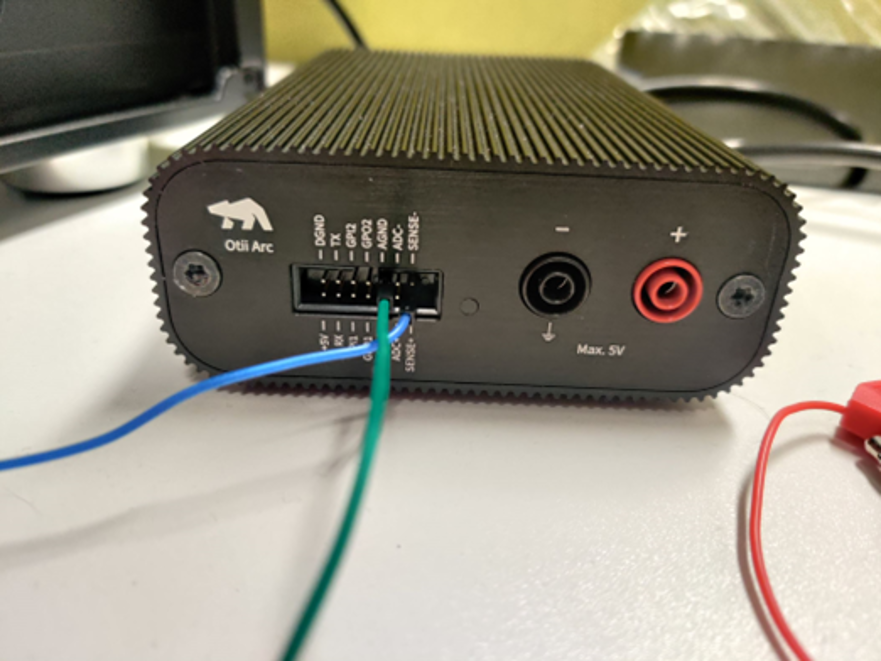
\includegraphics{Images/Picture2.png}} \\
    (a) & (b) \\
    \end{tabular}
    \caption[Clamp Power Measurement]{(a) Power Measurement using Current Clamp, (b) Connected to a Data Logger at 4 Kilo Samples Per Second.}
    \label{fig:Clamp}
\end{figure}

Two common methods used for measuring power are software and hardware based. Accurate power estimation is always challenging for software tools because they have to assume various factors in their models. Additionally, Taking the instantaneous power or TDP of a device is not accurate since power consumption varies on the specific workload. Therefore, measuring power over the time it takes for the algorithm to execute improves accuracy as opposed to using just fixed Wattage. 
The hardware measurement approach uses a current clamp meter shown in \ref{fig:Clamp}, which outputs a voltage for every Amp measured. The \textit{Otii Arc Pro}\cite{qoitech_2023} data-logger captures the time series data from the current clamp and generates a graph showing the current consumption over time. A script is developed to start and stop the measurements during the algorithm's execution. The mean current is averaged and multiplied by the input voltage to determine the energy consumed in Joules (J). 

The energy consumption is obtained using Eq. (\ref{eq:Energy}) where \textit{E} is energy, \textit{P} represents power and \textit{t} time.

\begin{equation}\label{eq:Energy}
E = P \times t
\end{equation}



\section{Experimental Results}
In this section, results of both CNN and SIFT algorithms implemented on a heterogeneous platform are observed and discussed in-depth.

\subsection{Heterogeneous SIFT Results}
In achieving that, a custom pipeline was created by targeting various algorithm components on different hardware based on their suitability obtained from the benchmarking framework. This includes the latency of transferring image data between memory and the accelerators. The heterogeneous architecture empowers the ability to pick and execute operations within the image processing algorithms on each architecture to meet the speed and power target. However, within the scope of this work, only an initial configuration of the SIFT algorithm is reported, which establishes preliminary steps toward future work on finding the most optimal configuration for the algorithms.
\begin{table}
\centering
\setlength{\extrarowheight}{0pt}
\addtolength{\extrarowheight}{\aboverulesep}
\addtolength{\extrarowheight}{\belowrulesep}
\setlength{\aboverulesep}{0pt}
\setlength{\belowrulesep}{0pt}
\caption{Execution Time (Excl. Memory Latency) on Individual Hardware and Heterogeneous Platform (CPU: 5900X, GPU: RTX-3070, FPGA: ZCU102). Baseline excludes memory latency. Incl. Memory Latency as additional data. }
\label{tab:heterogenoussummary}
\arrayrulecolor{black}
\resizebox{\linewidth}{!}{%
\begin{tabular}{c|c|c|c|c|c|c} 
\toprule
\rowcolor[rgb]{0.753,0.753,0.753} {\cellcolor[rgb]{0.753,0.753,0.753}} & \multicolumn{3}{c|}{\textbf{Baseline (ms)}} & \multicolumn{3}{c}{\textbf{Heterogeneous Architecture (ms)}} \\ 
\hhline{>{\arrayrulecolor[rgb]{0.753,0.753,0.753}}->{\arrayrulecolor{black}}------}
\rowcolor[rgb]{0.753,0.753,0.753} \multirow{-2}{*}{{\cellcolor[rgb]{0.753,0.753,0.753}}\textbf{Algorithm}} & \textbf{CPU} & \textbf{GPU} & \textbf{FPGA} & \textbf{Accelerator} & \textbf{Excl. Memory Latency} & \textbf{Inc. Memory Latency} \\ 
\cline{1-1}\cmidrule{2-2}\cline{3-3}\cmidrule{4-6}\cline{7-7}
RGB2Gray & 0.80 & 0.54 & 0.40 & CPU & 0.64 & 0.78 \\ 
\cmidrule{1-6}\cline{7-7}
\begin{tabular}[c]{@{}c@{}}Gaussian\\ Pyramid\end{tabular} & 684 & 3 & 6 & GPU & 3 & 115 \\ 
\cmidrule{1-6}\cline{7-7}
\begin{tabular}[c]{@{}c@{}}Extrema\\ Detection\end{tabular} & 112 & 2 & 3 & GPU & 2 & 101 \\ 
\cmidrule{1-6}\cline{7-7}
\begin{tabular}[c]{@{}c@{}}Orientation \textbackslash{}\textbackslash{}\& \\ Magnitude\end{tabular} & 97 & 4 & 2 & FPGA & 2 & 2 \\ 
\cmidrule{1-6}\cline{7-7}
\begin{tabular}[c]{@{}c@{}}Descriptor\\ Generation\end{tabular} & 21 & 1 & 1 & FPGA & 1 & 1 \\ 
\hhline{-------}
\rowcolor[rgb]{0.902,0.902,0.902} Total Runtime & 896.8 & 10.54 & 12.4 & CPU+GPU+FPGA & 8.64 & {\cellcolor[rgb]{0.898,0.898,0.898}}219.78 \\
\bottomrule
\end{tabular}
}
\end{table}

% \begin{table}[t]
% \caption{Execution time on individual hardware and heterogeneous platform.}
% \label{tab:heterogenoussummary}
% \resizebox{\textwidth}{!}{%
% \begin{tabular}{c|ccc|ccc}
% \toprule
%  & \multicolumn{3}{c|}{\textbf{Baseline (ms)}} & \multicolumn{3}{c}{\textbf{Heterogeneous Architecture (ms)}} \\ \cline{2-7}  
% \multirow{-2}{*}{\textbf{Algorithm}} & \multicolumn{1}{c|}{\textbf{CPU}} & \multicolumn{1}{c|}{\textbf{GPU}} & \textbf{FPGA} & \multicolumn{1}{c|}{\textbf{Accelerator}} & \multicolumn{1}{c|}{\textbf{Inc. Memory Latency}} & \textbf{Excl. Memory Latency} \\ \midrule
% RGB2Gray & \multicolumn{1}{c|}{0.80} & \multicolumn{1}{c|}{0.54} & 0.40 & \multicolumn{1}{c|}{CPU} & \multicolumn{1}{c|}{1} &  \\ \midrule
% \begin{tabular}[c]{@{}c@{}}Gaussian\\ Pyramid\end{tabular} & \multicolumn{1}{c|}{684} & \multicolumn{1}{c|}{3} & 4.5 & \multicolumn{1}{c|}{FPGA} & \multicolumn{1}{c|}{0} & 0 \\ \midrule
% \begin{tabular}[c]{@{}c@{}}Extrema\\ Detection\end{tabular} & \multicolumn{1}{c|}{112} & \multicolumn{1}{c|}{2} & 3 & \multicolumn{1}{c|}{FPGA} & \multicolumn{1}{c|}{0} & 0 \\ \midrule
% \begin{tabular}[c]{@{}c@{}}Orientation & \\ Magnitude\end{tabular} & \multicolumn{1}{c|}{97} & \multicolumn{1}{c|}{1} & 2 & \multicolumn{1}{c|}{GPU} & \multicolumn{1}{c|}{0} & 0 \\ \midrule
% \begin{tabular}[c]{@{}c@{}}Descriptor\\ Generation\end{tabular} & \multicolumn{1}{c|}{21} & \multicolumn{1}{c|}{1} & 1 & \multicolumn{1}{c|}{GPU} & \multicolumn{1}{c|}{0} & 0 \\ \midrule
% \rowcolor[HTML]{C0C0C0} 
% \multicolumn{1}{l|}{\cellcolor[HTML]{C0C0C0}Total Runtime} & \multicolumn{1}{c|}{\cellcolor[HTML]{C0C0C0}{\color[HTML]{000000} 896}} & \multicolumn{1}{c|}{\cellcolor[HTML]{C0C0C0}{\color[HTML]{000000} 7}} & {\color[HTML]{000000} 11} & \multicolumn{1}{c|}{\cellcolor[HTML]{C0C0C0}CPU+GPU+FPGA} & \multicolumn{1}{c|}{\cellcolor[HTML]{C0C0C0}{\color[HTML]{000000} 0}} & \cellcolor[HTML]{C0C0C0}{\color[HTML]{000000} 0} \\ \bottomrule
% \end{tabular}%
% }
% \end{table}   

\subsubsection{Heterogeneous SIFT Runtime \& Energy Consumption}

Table~\ref{tab:heterogenoussummary} shows the execution time of the SIFT algorithm on a heterogeneous platform. The table includes memory transfer latency between the host and devices, an aspect frequently overlooked in similar analyses. The results reveal that the heterogeneous platform (Excl. Memory Transfer) outperforms all discrete architectures, CPU, GPU and FPGA by $103\times$, $1.21\times$ and $1.43\times$, respectively. However, taking data transfer into account, the heterogeneous architecture increases in execution time due to host task scheduling. On the other hand, As accelerators are fabricated on the same silicon die, memory latency would significantly be reduced.

\begin{figure}[tb]
    \centering
\resizebox{\linewidth}{!}{\begin{tikzpicture}
  \begin{axis}[                    
  ybar,    
  ymin=0,
  ymode=log,
  scaled y ticks=false,  
  width=\columnwidth,  
  legend image code/.code={ \draw[#1, draw=none] (0cm,-0.1cm) rectangle (0.5cm,0.3cm);},
  legend style={
    at={(0.70,0.99)},
    anchor=north,
    legend columns=2,
    draw=black,
    fill=white,
    thick
  },
  ylabel={Power Consumption (Joules)},
  symbolic x coords={Total,RGB2Gray,Gaussian Pyramid,Extrema Detect,Orientation \& Magnitude,Descriptor Generation},
  xtick=data,
  nodes near coords,
  scaled x ticks=false,
  nodes near coords style={
    font=\normalsize,
    anchor=west,
    rotate=90,
    inner xsep=1pt,
    /pgf/number format/.cd,
    fixed,
    precision=2,
    /tikz/every node/.append style={xshift=0.2cm}
  },
  enlarge x limits=0.09,
  bar width=0.35cm,
  x tick label style={
    align=center,   % enable text wrapping
    text width=1.5cm  % set the text width
  }
  ]
  \addplot[pattern=north west lines,pattern color=black, fill=blue!20, postaction={pattern=north east lines}] coordinates {(Total, 80640)(RGB2Gray,72)(Gaussian Pyramid, 64980)(Extrema Detect, 8400)(Orientation \& Magnitude, 7760)(Descriptor Generation, 1575)};%CPU
  
  \addplot[pattern=north east lines,pattern color=black,fill=green!40, postaction={pattern=dots}] coordinates {(Total,540.46)(RGB2Gray,18.9)(Gaussian Pyramid, 240)(Extrema Detect, 80)(Orientation \& Magnitude, 180)(Descriptor Generation, 43)};%GPU
 
  \addplot[pattern=dots,pattern color=black,fill=red!30, postaction={pattern=grid}] coordinates {(Total, 403.2) (RGB2Gray,9.72) (Gaussian Pyramid, 192)(Extrema Detect, 55)(Orientation \& Magnitude, 36)(Descriptor Generation,29)};%FPGA

  \addplot[pattern=horizontal lines,pattern color=black,fill=brown!30, postaction={pattern=horizontal lines}] coordinates {(Total, 442.4) (RGB2Gray,51.2) (Gaussian Pyramid, 220)(Extrema Detect, 72)(Orientation \& Magnitude, 53)(Descriptor Generation,32)};%HP

  \legend{CPU: 5900X,GPU: 3070,FPGA: ZCU106, Heterogeneous}
  \end{axis}
\end{tikzpicture}
}    %\caption{Execution times for individual and combined algorithms.}
    \caption[SIFT Power Consumption]{SIFT Power Consumption, Baseline Homogeneous and Heterogeneous Implementation Comparison.}
    \label{fig:SIFTPower}
\end{figure}

The energy consumption results in \Fig{SIFTPower} reveal that the CPU consumes the most energy for all operation stages in \textit{SIFT} and \texttt{RGB2Gray} while the FPGA used the least. The \texttt{Gaussian Pyramid} stage stands out as the most energy intensive due to the substantial number of operations it requires. In contrast, the low resource requirements of \texttt{RGB2Gray} and \texttt{Descriptor Generation} stages reflected lower energy usage.

The heterogeneous architecture, which combines CPU, GPU and FPGA resources, strikes a balance between power consumption and execution time. The "\textit{Total}" power consumption is notably lower than the CPU but between both GPU and FPGA since the static power of other accelerators is taken into account.



\section{Heterogeneous CNN Results}
The results in \Fig{Resnet18PowerRuntime} \& \Fig{MobilenetPowerRuntime} show the total run-time and energy consumption of  Resnet18 and MobilenetV2 on each architecture and heterogeneous platform while \Fig{InferenceFPS} shows the inference in \textit{Frames per Second}. The tables \ref{tab:Mobilenet-V2 Result Summary} \& \ref{tab:ResNet-18 Result Summary}, summarises the results for the \textit{Total Execution Time}, \textit{Inference}, \textit{Convolution}, \textit{Fully Connected}, \textit{Total Energy}, \textit{CPU Energy}, \textit{Device Energy} \& \textit{Datalogger}

%for CPU, Accelerator, Sum of CPU + Accelerator and energy consumption recorded by the Data-logger.


\subsection{Inference}
\begin{figure}[t]
    \centering
\resizebox{\linewidth}{!}{\begin{tikzpicture}
\pgfplotsset{width=\textwidth,compat=1.3}
\begin{axis}[
    legend style={},
    ybar=1pt,
    ymin=0,
    bar width =15pt,
    legend image code/.code={\draw[#1, draw=none] (0cm,-0.1cm) rectangle (0.3cm,0.1cm);
                },
    ymajorgrids = true,
    legend style={at={(-0.000001,0.915)},
                   anchor=west,legend columns=1},
    ylabel={Frames per Second (FPS)},
    symbolic x coords={i9-9900K, 5900x(+), 3070(+), Xavier NX(-), Artix-7(-), ZCU106(+), HP(+), LP(-)},
    xtick=data,
    nodes near coords,
    nodes near coords style={font=\medium, anchor=west,rotate=90,inner
    xsep=0.5pt},
    x tick label style = { rotate=45, anchor=east},
    xlabel style={font=\large},
    ]

\addplot [fill=red!30] coordinates {(i9-9900K, 47)(5900x(+), 45)(3070(+), 250)(Xavier NX(-), 78) (Artix-7(-), 14.2)(ZCU106(+), 238)(HP(+), 270)(LP(-), 83)};%Resnet

\addplot [fill=blue!30]  coordinates {(i9-9900K, 43)(5900x(+), 40)(3070(+), 208)(Xavier NX(-), 56) (Artix-7(-), 10.2)(ZCU106(+), 217)(HP(+), 243)(LP(-), 68) };%Mobilenet

\legend{Resnet-18,Mobilenet-V2}
\end{axis}
\end{tikzpicture}
}    %\caption{Execution times for individual and combined algorithms.}
    \caption[Frames per Second (FPS) for Inference]{Frames per Second (FPS) for Inference on CPU:(I9-9900K, 5900X) GPU:(GTX 3070, Xavier NX) FPGA:(Artix-7, ZCU106), High-Power (HP), Low-Power (LP). (+) Denotes components in HP Platform, (-) Denotes Components in LP Platform.}
    \label{fig:InferenceFPS}
\end{figure}

According to \Fig{InferenceFPS}, \textit{Resnet18} CNN had the highest FPS value at $270$ in contrast to \textit{MobileNetV2} $243$ FPS on high and low power heterogeneous architecture. This difference in FPS can be attributed to the network depths and parameters, with \textit{ResNet-18} having $18$ layers and \textit{MobileNetV2} having $53$ layers, leading to differences in computational complexity. Considering individual hardware only, the '3070' GPU achieved the highest FPS on \textit{Resenet18} and the 'ZCU106' FPGA  for \textit{MobileNetv2}. On the other hand, the Artix-7 has the lowest FPS in both architectures due to limited resources and clock speed. In the case of both heterogeneous systems, \textit{HP} \& \textit{LP} architectures achieve higher FPS than their individual counterparts. 



\subsection{Total Execution Time}

\begin{figure}[t]
    \centering
\resizebox{0.9\columnwidth}{!}{\begin{tikzpicture}
\begin{axis}[   
xlabel={Total Runtime (s)},   
ylabel={Energy Consumption (Joules)},   
width=\columnwidth,        
ymin=0,    
xmin=0, 
grid=major,    
legend style={at={(0.77,1)},anchor=north}, anchor=west, legend columns=3, font=\small   ]

\addplot[only marks, mark=square*, mark size=3pt,mark options={pattern=crosshatch}, blue] coordinates {
        
        (0.25, 20.035)
    };
\addlegendentry{i9-11900KF}

\addplot[only marks, mark=square*, mark size=3pt, red] coordinates {
        (0.29,24.4267)

    };
\addlegendentry{5900x}

\addplot[only marks, mark=triangle*, mark size=3pt, mark options={pattern=crosshatch}, green] coordinates {
        (0.18, 19.754)

    };
\addlegendentry{3070}


\addplot[only marks, mark=o, mark size=3pt, black] coordinates {
        (0.74, 13.58)

    };
\addlegendentry{Xavier NX}

\addplot[only marks, mark=pentagon*, mark size=3pt, mark options={pattern=crosshatch}, orange] coordinates {
        (1.4, 6.1)

    };
\addlegendentry{Artix-7}

\addplot[only marks, mark=pentagon*, mark size=3pt, mark options={pattern=north east lines}, teal] coordinates {
        (0.19, 9.12)
    };
\addlegendentry{ZCU106}
\addplot[only marks, mark=asterisk, mark size=3pt, magenta] coordinates {
        (0.17, 8.93)
    };
\addlegendentry{HP}

\addplot[only marks, mark=+, mark size=3pt, black] coordinates {
        (0.62, 5.9)
    };
\addlegendentry{LP}


\end{axis}
\end{tikzpicture}
}    
    \caption[ResNet18 Energy Consumption]{{ResNet18 Energy Consumption \& Total Runtime Comparison; CPU:(I9, 5900X), GPU:(3070, Xavier NX), FPGA:(Artix-7, ZCU106), High-Power (HP), Low-Power (LP).}}
    \label{fig:Resnet18PowerRuntime}
\end{figure}

\begin{figure}[t]
    \centering
\resizebox{0.9\columnwidth}{!}{\begin{tikzpicture}
\begin{axis}[
xlabel={Total Runtime (s)},
ylabel={Energy Consumption (Joules)},
width=\columnwidth,
ymin=0,
%ymax=30,
xmin=0,
%xmax=1.5,
grid=major,
legend style={at={(0.77,1)},anchor=north}, legend columns=3, legend image post style={scale=1.7}, font=\small ]


\addplot[only marks, mark=square*, mark size=3pt,mark options={pattern=crosshatch}, blue] coordinates {
(0.28, 24.4)
};
\addlegendentry{i9}

\addplot[only marks, mark=square*, mark size=3pt, red] coordinates {
(0.31, 25.3)
};
\addlegendentry{5900x}

\addplot[only marks, mark=triangle*, mark size=3pt, mark options={pattern=crosshatch}, green] coordinates {
(0.231, 21.93)
};
\addlegendentry{3070}

\addplot[only marks, mark=o, mark size=3pt, black] coordinates {
(0.79, 15.28)
};

\addlegendentry{Xavier NX}

\addplot[only marks, mark=pentagon*, mark size=3pt, mark options={pattern=crosshatch}, orange] coordinates {
(0.99, 7.32)
};
\addlegendentry{Artix-7}

\addplot[only marks, mark=pentagon*, mark size=3pt, mark options={pattern=north east lines}, teal] coordinates {
(0.20, 10.55)
};
\addlegendentry{ZCU106}

\addplot[only marks, mark=asterisk, mark size=3pt, magenta] coordinates {
(0.19, 9.89)
};
\addlegendentry{HP}

\addplot[only marks, mark=+, mark size=3pt, black] coordinates {
(0.74, 6.80)
};
\addlegendentry{LP}

\end{axis}
\end{tikzpicture}

}    
    \caption[MobileNetV2 Energy Consumption]{MobileNetV2 Energy Consumption \& Total Runtime Comparison; CPU:(I9, 5900X), GPU:(3070, Xavier NX), FPGA:(Artix-7, ZCU106), High-Power (HP), Low-Power (LP).}
    \label{fig:MobilenetPowerRuntime}
\end{figure}



Regarding \Fig{Resnet18PowerRuntime} for Resnet18, it can be observed that the Artix-7 exhibits the highest total execution time, taking approximately $1.1$ seconds to complete the task. Conversely, the 'GPU: 3070' has the lowest real execution time, both completing the task at approximately $0.18$s. As for MobileNetV2 in \ref{fig:MobilenetPowerRuntime}, the 'FPGA: Artix-7' platform also leads with the highest execution time at $1.4$s, while the ZCU102 classifies the image in $0.19$s and GPU at $0.23$s. It is noteworthy to mention that the higher runtimes observed for the GPUs may be attributed to the communication and transfer of data from the CPU and lower core utilisation.

%In \Fig{executiontimeenergy} for Resnet18, the Artix-7 has the longest execution time at around 1.1 seconds, while the U50 and 3070 have the shortest at about 0.18 seconds. For MobileNetV2, the Artix-7 takes 1.4 seconds, while the Alveo U50 and Xilinx ZCU102 have the lowest execution times at 0.17 seconds and 0.19 seconds, respectively. High GPU runtimes may be due to data communication and transfer from the CPU.

%Artix-7 has the highest total execution time, taking approximately $1.1$s to complete the task. In contrast, the U50 \& 3070 have the lowest total execution time, both completing the task in approximately $0.18$s. In the case of MobileNetV2, while the Artix-7 leads with $1.4$s execution time, both Alveo U50 \& ZCU102 have the lowest at $0.17$s and $0.19$s respectively. However, the GPUs high runtimes is due to the communication and transfer of data from the CPU.

Total Execution time speedups of high (HP) and Low (LP) power systems are compared against their fastest discrete components within each system. The 'HP' system demonstrated a speedup of $1.05\times$ over the 'GPU:3070' for \textit{Resnet18} and $1.05\times$ for\textit{MobileNetv2}. In the case for 'LP' system, it exhibited a speedup of $1.21\times$ over the 'GPU: Xavier NX' for \textit{Resnet18} and $1.06\times$ for \textit{MobileNetv2}. The \texttt{Convolution} layer results show that the most time is spent performing convolution operations. However, taking in account data/memory transfer latency, both heterogeneous architectures implementations have interconnect (PCIe) and distance bottlenecks. This bottleneck reduces the FPS of HP \& LP systems by $10 \sim 25$ which in turn allows the 'GPU:3070' to marginally edge out on the HP system. The disparity between the \texttt{Total Wallclock} and \texttt{Inference} runtimes are due to the overhead and initialisation time which include model/weight loading and data preprocessing. In addition, the \texttt{Fully Connected} layer revealed that all architecture had comparable performance due to the layer's simple MAC operations.  

\subsection{Energy Consumption}
Concerning energy consumption, the discrete '5900 \& I9' CPUs consume the most energy in both CNN architectures, around $20\sim26$ Joules. The least amount of energy consumed is from both FPGA architectures, 'FPGA: Artix' and 'FPGA: ZCU106', which used less than $15$ Joules for both networks. Taking CPU idle energy usage into account results in GPUs having comparable energy usage statistics with both CPUs which is linked to higher CPU-GPU data transfer and initialisation cost. However, HP and LP systems consume $1.02\times$ and $1.03\times$ less energy, respectively, compared to the single ZCU106 and Artix architectures for \textit{Resnet18}. As for \textit{MobileNetV2}, there is a $1.06\times$ and $1.07\times$ reduction in energy consumption for the 'HP' and 'LP' systems, respectively. The idle accelerators within heterogeneous systems had their clocks lowered to save on static energy consumption. However, a small increase in idle energy usage was observed during execution. If idle energy is taken into account, then the energy consumption results of both HP \& LP systems would be greater than discrete FPGA but lower than GPU.

\begin{table}[]
\centering
\setlength{\extrarowheight}{0pt}
\addtolength{\extrarowheight}{\aboverulesep}
\addtolength{\extrarowheight}{\belowrulesep}
\setlength{\aboverulesep}{0pt}
\setlength{\belowrulesep}{0pt}
\caption{ResNet-18: Result Summary of Energy Consumption and Execution Time on Each Architecture. (Bold: Best Runtime Performance)}
\label{tab:ResNet-18 Result Summary}
\arrayrulecolor{black}
\resizebox{\textwidth}{!}{%
\begin{tabular}{c|c|c|c|c|c|c|c|c} 
\toprule
\rowcolor[rgb]{0.753,0.753,0.753} {\cellcolor[rgb]{0.753,0.753,0.753}} & \multicolumn{4}{c|}{\textbf{Execution time (s)}} & {\cellcolor[rgb]{0.753,0.753,0.753}} & {\cellcolor[rgb]{0.753,0.753,0.753}} & {\cellcolor[rgb]{0.753,0.753,0.753}} & {\cellcolor[rgb]{0.753,0.753,0.753}} \\ 
\hhline{>{\arrayrulecolor[rgb]{0.753,0.753,0.753}}->{\arrayrulecolor{black}}---->{\arrayrulecolor[rgb]{0.753,0.753,0.753}}----}
\rowcolor[rgb]{0.753,0.753,0.753} \multirow{-2}{*}{{\cellcolor[rgb]{0.753,0.753,0.753}}\textbf{Accelerator}} & Total Execution time & Inference & Convolution & Fully Connected & \multirow{-2}{*}{{\cellcolor[rgb]{0.753,0.753,0.753}}\begin{tabular}[c]{@{}>{\cellcolor[rgb]{0.753,0.753,0.753}}c@{}}\textbf{Sum CPU + Device}\\\textbf{ (Joule)}\end{tabular}} & \multirow{-2}{*}{{\cellcolor[rgb]{0.753,0.753,0.753}}\begin{tabular}[c]{@{}>{\cellcolor[rgb]{0.753,0.753,0.753}}c@{}}\textbf{Total CPU}\\\textbf{ (Joule)}\end{tabular}} & \multirow{-2}{*}{{\cellcolor[rgb]{0.753,0.753,0.753}}\begin{tabular}[c]{@{}>{\cellcolor[rgb]{0.753,0.753,0.753}}c@{}}\textbf{Total Device}\\\textbf{ (Joule)}\end{tabular}} & \multirow{-2}{*}{{\cellcolor[rgb]{0.753,0.753,0.753}}\begin{tabular}[c]{@{}>{\cellcolor[rgb]{0.753,0.753,0.753}}c@{}}\textbf{Datalogger }\\\textbf{ (Joule)}\end{tabular}} \\ 
\arrayrulecolor{black}\midrule
CPU: (i9-11900KF) & 0.25 & 0.021 & 0.019 & 0.0009 & 20.035 & 20.04 & N/A & 18.23 \\ 
\midrule
CPU: (5900X) & 0.29 & 0.022 & 0.018 & 0.0009 & 24.43 & 24.4267 & N/A & 22.48 \\ 
\midrule
GPU: (GTX 3070) & 0.18 & 0.004 & 0.0028 & 0.008 & 19.08 & 8.7 & 10.38 & 9.11 \\ 
\midrule
Jetson (Xavier NX) & 0.74 & 0.0128 & 0.0109 & 0.001 & 13.58 & N/A & 13.5716 & 10.56 \\ 
\midrule
FPGA: (ARCTIX7) & 1.1 & 0.070 & 0.062 & 0.0009 & 6.10 & N/A & 6.10 & 5.8 \\ 
\midrule
FPGA: (ZCU106) & 0.19 & 0.0042 & 0.0033 & 0.0009 & 9.12 & N/A & 9.12 & 8.07 \\ 
\midrule
\rowcolor[rgb]{0.894,0.894,0.894} 5900x + 3070 + ZCU106 & \textbf{\uline{0.17}} & 0.0037 & 0.0027 & 0.0009 & 8.93 & $\sim$ & $\sim$ & 8.5 \\ 
\midrule
\rowcolor[rgb]{0.894,0.894,0.894} ARM + Xavier +   Artix-7 & \textbf{\uline{0.62}} & 0.012 & 0.011 & 0.0009 & 5.90 & $\sim$ & $\sim$ & 5.44 \\
\bottomrule
\end{tabular}
}
\end{table}
\begin{table}[]
\centering
\setlength{\extrarowheight}{0pt}
\addtolength{\extrarowheight}{\aboverulesep}
\addtolength{\extrarowheight}{\belowrulesep}
\setlength{\aboverulesep}{0pt}
\setlength{\belowrulesep}{0pt}
\caption{Mobilenet-V2: Result Summary of Energy Consumption and Execution Time on Each Architecture. (Bold: Best Runtime Performance)}
\label{tab:Mobilenet-V2 Result Summary}
\arrayrulecolor{black}
\resizebox{\textwidth}{!}{%
\begin{tabular}{c|c|c|c|c|c|c|c} 
\toprule
\rowcolor[rgb]{0.753,0.753,0.753} {\cellcolor[rgb]{0.753,0.753,0.753}} & \multicolumn{3}{c|}{\textbf{Execution time (s)}} & {\cellcolor[rgb]{0.753,0.753,0.753}} & {\cellcolor[rgb]{0.753,0.753,0.753}} & {\cellcolor[rgb]{0.753,0.753,0.753}} & {\cellcolor[rgb]{0.753,0.753,0.753}} \\ 
\hhline{>{\arrayrulecolor[rgb]{0.753,0.753,0.753}}->{\arrayrulecolor{black}}--->{\arrayrulecolor[rgb]{0.753,0.753,0.753}}----}
\rowcolor[rgb]{0.753,0.753,0.753} \multirow{-2}{*}{{\cellcolor[rgb]{0.753,0.753,0.753}}\textbf{Accelerator}} & Total wallclock time & Inference & Convolution & \multirow{-2}{*}{{\cellcolor[rgb]{0.753,0.753,0.753}}\begin{tabular}[c]{@{}>{\cellcolor[rgb]{0.753,0.753,0.753}}c@{}}\textbf{Sum CPU + Device}\\\textbf{ (Joule)}\end{tabular}} & \multirow{-2}{*}{{\cellcolor[rgb]{0.753,0.753,0.753}}\begin{tabular}[c]{@{}>{\cellcolor[rgb]{0.753,0.753,0.753}}c@{}}\textbf{Total CPU}\\\textbf{ (Joule)}\end{tabular}} & \multirow{-2}{*}{{\cellcolor[rgb]{0.753,0.753,0.753}}\begin{tabular}[c]{@{}>{\cellcolor[rgb]{0.753,0.753,0.753}}c@{}}\textbf{Total Device}\\\textbf{ (Joule)}\end{tabular}} & \multirow{-2}{*}{{\cellcolor[rgb]{0.753,0.753,0.753}}\begin{tabular}[c]{@{}>{\cellcolor[rgb]{0.753,0.753,0.753}}c@{}}\textbf{Datalogger }\\\textbf{ (Joule)}\end{tabular}} \\ 
\arrayrulecolor{black}\midrule
CPU: (i9-11900KF) & 0.28 & 0.023 & 0.02 & 24.4 & 24.4 & N/A & 20.23 \\ 
\midrule
CPU: (5900X) & 0.31 & 0.025 & 0.022 & 25.3 & 25.3 & N/A & 21.48 \\ 
\midrule
GPU: (GTX 3070) & 0.231 & 0.0048 & 0.0045 & 21.945 & 9.24 & 12.70 & 19.43 \\ 
\midrule
Jetson (Xavier NX) & 0.79 & 0.018 & 0.0125 & 15.28 & N/A & 15.28 & 14.92 \\ 
\midrule
FPGA: (ARCTIX7) & 1.4 & 0.098 & 0.088 & 7.32 & N/A & 7.32 & 6.24 \\ 
\midrule
FPGA: (ZCU106) & 0.20 & 0.0046 & 0.0036 & 10.55 & N/A & 10.55 & 9.65 \\ 
\midrule
\rowcolor[rgb]{0.898,0.898,0.898} 5900x + 3070 + ZCU106 & \textbf{\uline{0.19}} & 0.0041 & 0.0029 & 9.89 & $\sim$ & $\sim$ & 9.01 \\ 
\midrule
\rowcolor[rgb]{0.898,0.898,0.898} ARM + Xavier +   Artix-7 & \textbf{\uline{0.74}} & 0.0145 & 0.015 & 6.80 & $\sim$ & $\sim$ & 5.86 \\
\bottomrule
\end{tabular}
}
\end{table}

\section{Conclusion}
In this chapter, partitioning strategies are introduced to map the layers of two widely used convolutional neural networks, namely, \texttt{Resnet18} and \texttt{Mobilnetv2}, along with a feature extraction algorithm (\texttt{SIFT}), onto a heterogeneous architecture. Two new CPU-GPU-FPGA systems, one designed for high performance and the other for low-power consumption, are proposed. The experiments demonstrate that when layer/per-operation partitioning methods are applied, both high-power and low-power systems outperform homogeneous accelerators in terms of energy efficiency and execution time. Furthermore, the results suggest that partitioning networks based on their layer profiles holds the potential for efficient deployment on heterogeneous architectures, offering a viable alternative to GPU/FPGA-only applications.


